% Options for packages loaded elsewhere
\PassOptionsToPackage{unicode}{hyperref}
\PassOptionsToPackage{hyphens}{url}
%
\documentclass[
]{article}
\usepackage{amsmath,amssymb}
\usepackage{lmodern}
\usepackage{iftex}
\ifPDFTeX
  \usepackage[T1]{fontenc}
  \usepackage[utf8]{inputenc}
  \usepackage{textcomp} % provide euro and other symbols
\else % if luatex or xetex
  \usepackage{unicode-math}
  \defaultfontfeatures{Scale=MatchLowercase}
  \defaultfontfeatures[\rmfamily]{Ligatures=TeX,Scale=1}
\fi
% Use upquote if available, for straight quotes in verbatim environments
\IfFileExists{upquote.sty}{\usepackage{upquote}}{}
\IfFileExists{microtype.sty}{% use microtype if available
  \usepackage[]{microtype}
  \UseMicrotypeSet[protrusion]{basicmath} % disable protrusion for tt fonts
}{}
\makeatletter
\@ifundefined{KOMAClassName}{% if non-KOMA class
  \IfFileExists{parskip.sty}{%
    \usepackage{parskip}
  }{% else
    \setlength{\parindent}{0pt}
    \setlength{\parskip}{6pt plus 2pt minus 1pt}}
}{% if KOMA class
  \KOMAoptions{parskip=half}}
\makeatother
\usepackage{xcolor}
\IfFileExists{xurl.sty}{\usepackage{xurl}}{} % add URL line breaks if available
\IfFileExists{bookmark.sty}{\usepackage{bookmark}}{\usepackage{hyperref}}
\hypersetup{
  pdftitle={ASPH305 Assignment 2},
  hidelinks,
  pdfcreator={LaTeX via pandoc}}
\urlstyle{same} % disable monospaced font for URLs
\usepackage{graphicx}
\makeatletter
\def\maxwidth{\ifdim\Gin@nat@width>\linewidth\linewidth\else\Gin@nat@width\fi}
\def\maxheight{\ifdim\Gin@nat@height>\textheight\textheight\else\Gin@nat@height\fi}
\makeatother
% Scale images if necessary, so that they will not overflow the page
% margins by default, and it is still possible to overwrite the defaults
% using explicit options in \includegraphics[width, height, ...]{}
\setkeys{Gin}{width=\maxwidth,height=\maxheight,keepaspectratio}
% Set default figure placement to htbp
\makeatletter
\def\fps@figure{htbp}
\makeatother
\setlength{\emergencystretch}{3em} % prevent overfull lines
\providecommand{\tightlist}{%
  \setlength{\itemsep}{0pt}\setlength{\parskip}{0pt}}
\setcounter{secnumdepth}{-\maxdimen} % remove section numbering
\ifLuaTeX
  \usepackage{selnolig}  % disable illegal ligatures
\fi

\title{ASPH305 Assignment 2}
\author{}
\date{}

\begin{document}
\maketitle

\hypertarget{asph305-homework-assignment-2}{%
\section{ASPH305 Homework Assignment
2:}\label{asph305-homework-assignment-2}}

\begin{center}\rule{0.5\linewidth}{0.5pt}\end{center}

\hypertarget{the-figure-below-shows-the-position-of-an-asteroid-as-seen-from-telescope-1-located-in-calgary-and-from-telescope-2-located-500km-away-from-telescope-1.-the-observations-were-taken-at-the-same-time.}{%
\subparagraph{\texorpdfstring{1: The figure below shows the position of
an asteroid as seen from telescope 1 (located in Calgary) and from
telescope 2 (located {\(500km\)} away from telescope 1). The
observations were taken at the same
time.}{1: The figure below shows the position of an asteroid as seen from telescope 1 (located in Calgary) and from telescope 2 (located 500km away from telescope 1). The observations were taken at the same time.}}\label{the-figure-below-shows-the-position-of-an-asteroid-as-seen-from-telescope-1-located-in-calgary-and-from-telescope-2-located-500km-away-from-telescope-1.-the-observations-were-taken-at-the-same-time.}}

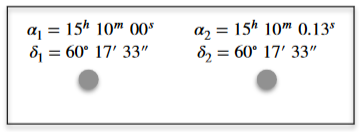
\includegraphics{C:/Users/maxst/sciencia/a2picture1.png}

\begin{quote}
\mbox{}%
\hypertarget{a.-calculate-the-distance-to-the-asteroid-in-au.-you-may-ignore-the-curvature-of-the-earth-and-the-exact-latitudelongitude-of-each-telescope.}{%
\subparagraph{\texorpdfstring{a.) Calculate the distance to the asteroid
(in {\(AU\)}). You may ignore the curvature of the Earth and the exact
latitude/longitude of each
telescope.}{a.) Calculate the distance to the asteroid (in AU). You may ignore the curvature of the Earth and the exact latitude/longitude of each telescope.}}\label{a.-calculate-the-distance-to-the-asteroid-in-au.-you-may-ignore-the-curvature-of-the-earth-and-the-exact-latitudelongitude-of-each-telescope.}}
\end{quote}

We can find the distance using the \emph{parallactic angle formula}:

\hypertarget{plbracktextradsrbrack-fracdd.}{%
\subsubsection{\texorpdfstring{{\[p\,\lbrack\text{rads}\rbrack = \frac{d}{D}.\]}}{p\textbackslash,\textbackslash lbrack\textbackslash text\{rads\}\textbackslash rbrack = \textbackslash frac\{d\}\{D\}.}}\label{plbracktextradsrbrack-fracdd.}}

Rearranging:

\hypertarget{d-fracdp.}{%
\subsubsection{\texorpdfstring{{\[D = \frac{d}{p}.\]}}{D = \textbackslash frac\{d\}\{p\}.}}\label{d-fracdp.}}

The declination {\(\delta\)} of the asteroid is the same as measured
from each telescope - therefore, the \emph{parallactic angle {\(p\)}}
can be found from the difference between the measured values for
\emph{right ascension}:

\hypertarget{beginmatrix-alpha_2---alpha_1-15h-10m-0.13s---15h-10m-0.0s-0.13s-0.13sleft-fracpi43200textradians-right-9.45387-times-10--6textrad.-endmatrix}{%
\subsubsection{\texorpdfstring{{\[\begin{matrix}
{\alpha_{2} - \alpha_{1}} & {= 15^{h}\, 10^{m}\, 0.13^{s} - 15^{h}\, 10^{m}\, 0.0^{s}} \\
 & {= 0.13^{s}} \\
 & {= 0.13^{s}\left( \frac{\pi}{43200}\text{~radians} \right)} \\
 & {= 9.45387 \times 10^{- 6}\text{~rad}.} \\
\end{matrix}\]}}{\textbackslash begin\{matrix\}
\{\textbackslash alpha\_\{2\} - \textbackslash alpha\_\{1\}\} \& \{= 15\^{}\{h\}\textbackslash, 10\^{}\{m\}\textbackslash, 0.13\^{}\{s\} - 15\^{}\{h\}\textbackslash, 10\^{}\{m\}\textbackslash, 0.0\^{}\{s\}\} \textbackslash\textbackslash{}
 \& \{= 0.13\^{}\{s\}\} \textbackslash\textbackslash{}
 \& \{= 0.13\^{}\{s\}\textbackslash left( \textbackslash frac\{\textbackslash pi\}\{43200\}\textbackslash text\{\textasciitilde radians\} \textbackslash right)\} \textbackslash\textbackslash{}
 \& \{= 9.45387 \textbackslash times 10\^{}\{- 6\}\textbackslash text\{\textasciitilde rad\}.\} \textbackslash\textbackslash{}
\textbackslash end\{matrix\}}}\label{beginmatrix-alpha_2---alpha_1-15h-10m-0.13s---15h-10m-0.0s-0.13s-0.13sleft-fracpi43200textradians-right-9.45387-times-10--6textrad.-endmatrix}}

However, this is actually \emph{twice} the parallactic angle, leaving us
with:

\hypertarget{p-frac9.45387-times-10--6textrad2-4.72693-times-10--6textrad.}{%
\subsubsection{\texorpdfstring{{\[p = \frac{9.45387 \times 10^{- 6}\text{~rad}}{2} = 4.72693 \times 10^{- 6}\text{~rad.}\]}}{p = \textbackslash frac\{9.45387 \textbackslash times 10\^{}\{- 6\}\textbackslash text\{\textasciitilde rad\}\}\{2\} = 4.72693 \textbackslash times 10\^{}\{- 6\}\textbackslash text\{\textasciitilde rad.\}}}\label{p-frac9.45387-times-10--6textrad2-4.72693-times-10--6textrad.}}

Now that we have the parallactic angle in radians, we need the baseline
distance in units of {\(AU\)} (recalling that the baseline is
\emph{half} the distance between the telescopes):

\hypertarget{km-1.33692-times-10--6-au.}{%
\subsubsection{\texorpdfstring{{\[250\, km = 1.33692 \times 10^{- 6}\, AU.\]}}{250\textbackslash, km = 1.33692 \textbackslash times 10\^{}\{- 6\}\textbackslash, AU.}}\label{km-1.33692-times-10--6-au.}}

We can now find the distance to the asteroid:

\begin{quote}
\hypertarget{d-fracdp-frac1.33692-times-10--6-au4.72693-times-10--6-0.28283-au.}{%
\subsubsection{\texorpdfstring{{\[D = \frac{d}{p} = \frac{1.33692 \times 10^{- 6}\, AU}{4.72693 \times 10^{- 6}} = 0.28283\, AU.\]}}{D = \textbackslash frac\{d\}\{p\} = \textbackslash frac\{1.33692 \textbackslash times 10\^{}\{- 6\}\textbackslash, AU\}\{4.72693 \textbackslash times 10\^{}\{- 6\}\} = 0.28283\textbackslash, AU.}}\label{d-fracdp-frac1.33692-times-10--6-au4.72693-times-10--6-0.28283-au.}}
\end{quote}

NASA identifies Potentially Hazardous Objects (PHOs) as near-Earth
objects whose orbit brings them within \textasciitilde0.05 {\(AU\)} of
Earth's orbit, so no cause for alarm yet.

\begin{center}\rule{0.5\linewidth}{0.5pt}\end{center}

\begin{quote}
\mbox{}%
\hypertarget{b.-at-the-time-of-the-above-observation-the-asteroid-is-moving-towards-us-with-a-velocity-of-36.056-kms-at-an-angle-of-30circ-with-respect-to-the-line-of-sight-i.e.-the-vector-between-earth-and-the-asteroid.-calculate-the-radial-and-tangential-velocity-components-in-kms-and-the-proper-motion-that-would-be-observed-from-earth-in-units-of-both-yr-and-min.}{%
\subparagraph{\texorpdfstring{b.) At the time of the above observation,
the asteroid is moving towards us with a velocity of {\(36.056\, km/s\)}
at an angle of {\(30{^\circ}\)} with respect to the line of sight
(\emph{i.e.} the vector between Earth and the asteroid). Calculate the
radial and tangential velocity components (in {\(km/s\)}), and the
proper motion that would be observed from Earth (in units of BOTH
\emph{"/yr} and
\emph{"/min}).}{b.) At the time of the above observation, the asteroid is moving towards us with a velocity of 36.056\textbackslash, km/s at an angle of 30\{\^{}\textbackslash circ\} with respect to the line of sight (i.e. the vector between Earth and the asteroid). Calculate the radial and tangential velocity components (in km/s), and the proper motion that would be observed from Earth (in units of BOTH "/yr and "/min).}}\label{b.-at-the-time-of-the-above-observation-the-asteroid-is-moving-towards-us-with-a-velocity-of-36.056-kms-at-an-angle-of-30circ-with-respect-to-the-line-of-sight-i.e.-the-vector-between-earth-and-the-asteroid.-calculate-the-radial-and-tangential-velocity-components-in-kms-and-the-proper-motion-that-would-be-observed-from-earth-in-units-of-both-yr-and-min.}}
\end{quote}

A diagram to illustrate:

\begin{verbatim}
    <svg xmlns="http://www.w3.org/2000/svg" class="role-diagram-draw-area" style="overflow: visible;"><g class="shapes-region" style="stroke: black; fill: none;"><g class="composite-shape"><path class="real" d=" M430.43,113.12 L438.98,110.9 L441.2,119.45 L432.65,121.67 Z" style="stroke-width: 1px; stroke: rgb(0, 0, 0); fill: none; fill-opacity: 1;"/></g><g class="arrow-line"><path class="connection real" stroke-dasharray="7.5 6" d="  M558.67,85.5 L452.09,173.29" style="stroke: rgb(0, 0, 0); stroke-opacity: 1; stroke-width: 2px; fill: none; fill-opacity: 1;"/><g stroke="none" fill="rgb(0,0,0)" fill-opacity="1" transform="matrix(0.7718465695580344,-0.6358088337397447,0.6358088337397447,0.7718465695580344,449,175.83332824707028)" style="stroke: none; fill: rgb(0, 0, 0); stroke-width: 2px;"><path d=" M11.61,-5.58 L0,0 L11.61,5.58 Z"/></g></g><g class="arrow-line"><path class="connection real" stroke-dasharray="" d="  M107.11,178.76 L558.67,85.5" style="stroke: rgb(0, 0, 0); stroke-width: 1px; fill: none; fill-opacity: 1;"/></g><g class="composite-shape"><defs><!-- react-text: 2585 --> <!-- /react-text --><radialGradient id="_pgflaew7vxt2dg-full-view" gradientTransform="matrix(1.28, 0, 0, 1.28, -0.14, -0.14)" cx="0.43" cy="0.38" fx="0.43" fy="0.38"><!-- react-text: 2587 --> <!-- /react-text --><stop offset="0" style="stop-color: rgb(153, 218, 255); stop-opacity: 1;"/><stop offset="0.39" style="stop-color: rgb(126, 211, 33); stop-opacity: 1;"/><stop offset="0.71" style="stop-color: rgb(33, 170, 211); stop-opacity: 1;"/><stop offset="0.95" style="stop-color: rgb(126, 211, 33); stop-opacity: 1;"/></radialGradient></defs><path class="real" d=" M54.64,178.76 C54.64,151.29 78.13,129.02 107.11,129.02 C136.09,129.02 159.58,151.29 159.58,178.76 C159.58,206.23 136.09,228.5 107.11,228.5 C78.13,228.5 54.64,206.23 54.64,178.76 Z" style="stroke-width: 1px; stroke: rgb(0, 0, 0); fill: url(&quot;#_pgflaew7vxt2dg-full-view&quot;); fill-opacity: 1;"/></g><g class="composite-shape"><path class="real" d=" M525.77,113.73 C523.58,111.15 521.62,108.31 519.95,105.22 C517.89,101.42 516.38,97.48 515.39,93.48 L563.67,81.53 Z" style="stroke-width: 1px; stroke: none; fill: none; fill-opacity: 1; stroke-opacity: 1;"/><path class="real" d=" M525.77,113.73 C523.58,111.15 521.62,108.31 519.95,105.22 C517.89,101.42 516.38,97.48 515.39,93.48" style="stroke-width: 1px; stroke: rgb(0, 0, 0); fill: none; fill-opacity: 1; stroke-opacity: 1;"/></g><g class="arrow-line"><path class="connection real" stroke-dasharray="6 6" d="  M107.11,129.02 L107.11,144.5 L107.11,212.5 L107.11,228.5" style="stroke: rgb(0, 0, 0); stroke-width: 1px; fill: none; fill-opacity: 1; stroke-opacity: 0.5;"/></g><g class="composite-shape"><path class="real" d=" M159.58,178.76 C155.07,186.1 133.51,191.36 107.71,190.91 C78.97,190.41 55.76,183.02 55.52,174.36 L107.98,175.05 Z" style="stroke-width: 1px; stroke: none; fill: none; fill-opacity: 1; stroke-dasharray: 6px, 6px; stroke-opacity: 0.5;"/><path class="real" d=" M159.58,178.76 C155.07,186.1 133.51,191.36 107.71,190.91 C78.97,190.41 55.76,183.02 55.52,174.36" style="stroke-width: 1px; stroke: rgb(0, 0, 0); fill: none; fill-opacity: 1; stroke-dasharray: 6px, 6px; stroke-opacity: 0.5;"/></g><g class="composite-shape"><path class="real" d=" M158.22,175.39 C152.83,169.94 131.93,166 107,166.2 C78.33,166.42 55.08,172.03 54.64,178.76 L107.1,178.57 Z" style="stroke-width: 1px; stroke: none; fill: none; fill-opacity: 1; stroke-dasharray: 1.125px, 3.35px; stroke-opacity: 0.26;"/><path class="real" d=" M158.22,175.39 C152.83,169.94 131.93,166 107,166.2 C78.33,166.42 55.08,172.03 54.64,178.76" style="stroke-width: 1px; stroke: rgb(0, 0, 0); fill: none; fill-opacity: 1; stroke-dasharray: 1.125px, 3.35px; stroke-opacity: 0.26;"/></g><g class="arrow-line"><path class="connection real" stroke-dasharray="" d="  M558.67,85.5 L573.07,145.94" style="stroke: rgb(74, 144, 226); stroke-width: 2px; fill: none; fill-opacity: 1; stroke-opacity: 1;"/><g stroke="none" fill="rgb(74,144,226)" transform="matrix(-0.2319176813831601,-0.9727354157538725,0.9727354157538725,-0.2319176813831601,574,149.8333282470703)" style="stroke: none; fill: rgb(74, 144, 226); stroke-width: 2px;" fill-opacity="1"><path d=" M13.4,-6.43 L0,0 L13.4,6.44 L8.9,0 Z"/></g></g><g class="arrow-line"><path class="connection real" stroke-dasharray="" d="  M557,87.07 L434.35,112.31" style="stroke: rgb(211, 0, 0); stroke-width: 2px; fill: none; fill-opacity: 1; stroke-opacity: 1;"/><g stroke="none" fill="rgb(211,0,0)" transform="matrix(0.9794698311727877,-0.20159079796049914,0.20159079796049914,0.9794698311727877,430.4315199830119,113.11883182991609)" style="stroke: none; fill: rgb(211, 0, 0); stroke-width: 2px;" fill-opacity="1"><path d=" M13.4,-6.43 L0,0 L13.4,6.44 L8.9,0 Z"/></g></g><g class="composite-shape"><defs><!-- react-text: 3644 --> <!-- /react-text --><radialGradient id="_pgf6q3pq57andg-full-view" gradientTransform="matrix(1, 0, 0, 1, 0, 0)" cx="0.5" cy="0.5" fx="0.5" fy="0.5"><!-- react-text: 3646 --> <!-- /react-text --><stop offset="0" style="stop-color: rgb(120, 135, 166); stop-opacity: 1;"/><stop offset="0.36" style="stop-color: rgb(71, 76, 87); stop-opacity: 1;"/><stop offset="1" style="stop-color: rgb(0, 0, 0); stop-opacity: 1;"/></radialGradient></defs><path class="real" d=" M563.67,85.78 C563.67,88.12 561.28,90.03 558.33,90.03 C555.39,90.03 553,88.12 553,85.78 C553,83.43 555.39,81.53 558.33,81.53 C561.89,81.53 563.67,81.53 563.67,81.53 C563.67,81.53 563.67,82.94 563.67,85.78 Z" style="stroke-width: 1px; stroke: rgb(0, 0, 0); fill: url(&quot;#_pgf6q3pq57andg-full-view&quot;); fill-opacity: 1;"/></g><g class="arrow-line"><path class="connection real" stroke-dasharray="1.125 3.35" d="  M449,175.83 L574,149.83" style="stroke: rgb(0, 0, 0); stroke-width: 1px; fill: none; fill-opacity: 1;"/></g><g class="arrow-line"><path class="connection real" stroke-dasharray="1.125 3.35" d="  M431.4,111.87 L440,146.83 L449,175.83" style="stroke: rgb(0, 0, 0); stroke-width: 1px; fill: none; fill-opacity: 1;"/></g><g class="composite-shape"><path class="real" d=" M478.76,169.49 C478.03,166.8 476.99,164.19 475.63,161.69 C474.74,160.05 473.74,158.49 472.63,157.03 L415.51,194.26 Z" style="stroke-width: 1px; stroke: none; stroke-opacity: 1; fill: none; fill-opacity: 1;"/><path class="real" d=" M478.76,169.49 C478.03,166.8 476.99,164.19 475.63,161.69 C474.74,160.05 473.74,158.49 472.63,157.03" style="stroke-width: 1px; stroke: rgb(0, 0, 0); stroke-opacity: 1; fill: none; fill-opacity: 1;"/></g><g/></g><g/><g/><g/></svg>
    <svg xmlns="http://www.w3.org/2000/svg" xmlns:xlink="http://www.w3.org/1999/xlink" width="700" height="300" style="width:700px;height:300px;font-family:Asana-Math, Asana;background:#FFF;"><g transform="matrix(0.9734592051865375,-0.22886060350701387,0.22886060350701387,0.9734592051865375,-21.56885920974753,68.62892510213061)"><g><g><g transform="matrix(1,0,0,1,249.33331298828125,132.89998779296874)"><path transform="matrix(0.0136,0,0,-0.0136,0,0)" d="M349 664L352 692L238 689C222 689 204 689 161 690L97 692L94 664L141 662C165 661 176 653 176 635L81 55C77 37 65 30 21 23L16 -3L57 -2C88 -1 150 0 170 0C170 0 467 -1 467 -1C467 -1 500 0 500 0C499 25 510 103 523 165L492 165L475 103C466 71 457 54 448 49C435 44 371 39 304 39C255 39 228 40 162 46C165 64 256 605 256 613C263 651 270 658 307 661ZM589 388L596 368L628 389C665 412 668 414 675 414C685 414 693 404 693 391C693 384 689 361 685 347L619 107C611 76 606 49 606 30C606 6 617 -9 636 -9C662 -9 698 12 796 85L786 103L760 86C731 67 708 56 699 56C692 56 686 66 686 76C686 86 688 95 693 116L770 420C774 437 776 448 776 456C776 473 767 482 751 482C729 482 692 461 617 408ZM783 712C754 712 725 679 725 645C725 620 740 604 764 604C795 604 819 633 819 671C819 695 804 712 783 712ZM856 388L863 368L895 389C932 412 935 414 942 414C953 414 960 404 960 389C960 338 919 145 878 2L885 -9C910 -2 933 4 955 8C974 134 995 199 1041 268C1095 352 1170 414 1215 414C1226 414 1232 405 1232 390C1232 372 1229 351 1221 319L1169 107C1160 70 1156 47 1156 31C1156 6 1167 -9 1186 -9C1212 -9 1248 12 1346 85L1336 103L1310 86C1281 67 1259 56 1249 56C1242 56 1236 65 1236 76C1236 81 1237 92 1238 96L1304 372C1311 401 1315 429 1315 446C1315 469 1304 482 1284 482C1242 482 1173 444 1114 389C1076 354 1048 320 996 247L1034 408C1038 426 1040 438 1040 449C1040 470 1032 482 1017 482C996 482 957 460 884 408ZM1715 111L1691 94C1638 56 1590 36 1554 36C1507 36 1478 73 1478 133C1478 158 1481 185 1486 214C1503 218 1612 248 1637 259C1722 296 1761 342 1761 404C1761 451 1727 482 1677 482C1609 496 1499 423 1462 349C1432 299 1402 180 1402 113C1402 35 1446 -11 1518 -11C1575 -11 1631 17 1723 92ZM1500 274C1517 343 1537 386 1566 412C1584 428 1615 440 1639 440C1668 440 1687 420 1687 388C1687 344 1652 297 1600 272C1572 258 1536 247 1491 237ZM2041 152C2041 46 2086 -11 2169 -11C2224 -11 2284 15 2329 57C2391 116 2435 230 2435 331C2435 425 2385 482 2302 482C2198 482 2041 382 2041 152ZM2265 444C2326 444 2359 399 2359 315C2359 219 2328 113 2284 60C2266 39 2240 27 2209 27C2151 27 2117 72 2117 151C2117 264 2156 387 2205 427C2218 438 2241 444 2265 444ZM2812 437L2796 437L2817 549C2833 635 2861 673 2907 673C2937 673 2964 658 2979 634L2989 638C2994 654 3004 685 3012 705L3017 720C3001 727 2970 733 2947 733C2936 733 2920 730 2912 726C2888 715 2806 654 2783 630C2761 608 2749 578 2738 521L2723 442C2682 422 2662 414 2637 405L2632 383L2713 383L2704 327C2674 132 2637 -54 2615 -123C2597 -182 2567 -213 2531 -213C2508 -213 2497 -206 2479 -184L2465 -188C2461 -211 2447 -259 2442 -268C2451 -273 2466 -276 2477 -276C2518 -276 2572 -245 2611 -198C2682 -114 2702 -18 2786 383L2890 383C2894 402 2901 425 2907 439L2903 446C2874 439 2875 437 2812 437ZM3297 148C3292 97 3286 62 3275 16C3313 -2 3347 -11 3382 -11C3431 -11 3477 7 3528 47C3579 87 3600 124 3600 174C3600 228 3568 257 3494 271L3451 279C3391 290 3372 307 3372 348C3372 401 3417 442 3474 442C3515 442 3553 424 3569 397L3569 342L3592 342C3596 377 3600 404 3611 455C3572 474 3544 482 3511 482C3459 482 3398 452 3350 404C3324 377 3313 352 3313 316C3313 260 3344 228 3410 215L3473 203C3517 195 3533 177 3533 138C3533 73 3487 29 3416 29C3381 29 3350 40 3322 64L3322 148ZM3688 388L3695 368L3727 389C3764 412 3767 414 3774 414C3784 414 3792 404 3792 391C3792 384 3788 361 3784 347L3718 107C3710 76 3705 49 3705 30C3705 6 3716 -9 3735 -9C3761 -9 3797 12 3895 85L3885 103L3859 86C3830 67 3807 56 3798 56C3791 56 3785 66 3785 76C3785 86 3787 95 3792 116L3869 420C3873 437 3875 448 3875 456C3875 473 3866 482 3850 482C3828 482 3791 461 3716 408ZM3882 712C3853 712 3824 679 3824 645C3824 620 3839 604 3863 604C3894 604 3918 633 3918 671C3918 695 3903 712 3882 712ZM4206 482C4139 482 3986 419 3986 259C3986 182 4031 136 4108 136C4116 136 4127 136 4138 137L4097 99C4081 84 4070 66 4070 52C4070 42 4077 31 4091 19C4022 -4 3894 -48 3894 -159C3894 -230 3964 -276 4073 -276C4202 -276 4315 -204 4315 -121C4315 -85 4294 -49 4251 -14L4191 35C4157 62 4144 81 4144 100C4144 114 4159 128 4171 146C4269 170 4340 253 4340 342C4340 357 4337 376 4336 380C4353 378 4361 378 4370 378C4387 378 4397 379 4420 382L4429 427L4426 433C4398 426 4378 424 4324 424C4324 425 4300 482 4206 482ZM4107 1L4184 -58C4230 -94 4249 -121 4249 -154C4249 -206 4180 -248 4097 -248C4015 -248 3958 -206 3958 -145C3958 -43 4068 -11 4107 1ZM4181 448C4239 448 4268 412 4268 341C4268 238 4220 168 4150 168C4089 168 4057 209 4057 288C4057 383 4108 448 4181 448ZM4666 722L4654 733C4609 711 4568 697 4494 691L4490 670L4538 670C4556 670 4572 667 4572 647C4572 641 4572 632 4570 622L4528 388C4508 272 4466 80 4440 2L4447 -9L4516 7C4524 64 4538 164 4578 236C4623 317 4726 414 4768 414C4779 414 4790 407 4790 393C4790 375 4785 342 4775 303L4724 107C4718 85 4711 55 4711 31C4711 6 4721 -9 4742 -9C4774 -9 4842 41 4901 85L4891 103L4865 86C4842 71 4816 56 4804 56C4797 56 4791 65 4791 76C4791 88 4794 101 4798 116L4862 372C4868 398 4873 423 4873 447C4873 464 4867 482 4841 482C4806 482 4729 437 4661 374C4628 343 4602 308 4574 273L4570 275ZM5054 390L4998 107C4997 99 4985 61 4985 31C4985 6 4996 -9 5015 -9C5050 -9 5085 11 5163 74L5194 99L5184 117L5139 86C5110 66 5090 56 5079 56C5070 56 5065 64 5065 76C5065 102 5079 183 5108 328L5121 390L5228 390L5239 440C5201 436 5167 434 5129 434C5145 528 5156 577 5174 631L5163 646C5143 634 5116 622 5085 610L5060 440C5016 419 4990 408 4972 403L4970 390Z" stroke="rgb(0,0,0)" stroke-opacity="1" stroke-width="8" fill="rgb(0,0,0)" fill-opacity="1"></path></g></g></g></g><g><g><g><g transform="matrix(1,0,0,1,89.66668701171875,248.53334045410156)"><path transform="matrix(0.017,0,0,-0.017,0,0)" d="M221 334L338 334L470 330L489 375L485 382C404 378 344 376 266 376L229 376L276 646C308 647 391 650 413 650C475 650 516 641 517 626L525 537L549 537C552 601 559 651 570 689C549 691 519 692 501 692C498 692 487 692 463 691L343 690C334 689 160 691 150 691L105 692L102 664L156 662C180 661 191 653 191 635C191 621 187 589 182 559L95 55C91 37 79 30 35 23L30 -3L71 -2C102 -1 164 0 184 0L409 -3C423 -3 448 -2 481 -1L514 0L518 36C520 56 525 86 534 135L539 161L512 161L496 101C486 65 477 53 455 48C435 44 362 39 308 39C267 39 240 40 171 46ZM881 204L852 77C848 60 846 42 846 26C846 4 855 -9 870 -9C893 -9 934 17 1016 85L1009 106C985 86 956 59 934 59C925 59 919 68 919 82C919 87 919 90 920 93L1012 472L1002 481L969 463C928 478 911 482 884 482C856 482 836 477 809 464C747 433 714 403 689 354C645 265 614 145 614 67C614 23 629 -11 648 -11C685 -11 765 41 881 204ZM929 414C907 305 888 253 854 201C797 117 736 59 704 59C692 59 686 72 686 99C686 163 714 280 749 360C773 415 796 433 844 433C867 433 885 429 929 414ZM1421 365C1424 403 1429 435 1437 476C1426 481 1422 482 1417 482C1386 482 1355 458 1319 407C1280 351 1241 291 1225 256L1257 408C1261 425 1263 438 1263 450C1263 470 1255 482 1240 482C1219 482 1181 461 1107 408L1079 388L1086 368L1118 389C1146 407 1157 412 1166 412C1176 412 1183 403 1183 390C1183 332 1140 126 1100 -2L1110 -9C1125 -4 1141 -1 1164 4L1177 6L1203 126C1221 209 1244 262 1288 319C1322 363 1349 384 1371 384C1386 384 1396 379 1407 365ZM1566 390L1510 107C1509 99 1497 61 1497 31C1497 6 1508 -9 1527 -9C1562 -9 1597 11 1675 74L1706 99L1696 117L1651 86C1622 66 1602 56 1591 56C1582 56 1577 64 1577 76C1577 102 1591 183 1620 328L1633 390L1740 390L1751 440C1713 436 1679 434 1641 434C1657 528 1668 577 1686 631L1675 646C1655 634 1628 622 1597 610L1572 440C1528 419 1502 408 1484 403L1482 390ZM2009 722L1997 733C1952 711 1911 697 1837 691L1833 670L1881 670C1899 670 1915 667 1915 647C1915 641 1915 632 1913 622L1871 388C1851 272 1809 80 1783 2L1790 -9L1859 7C1867 64 1881 164 1921 236C1966 317 2069 414 2111 414C2122 414 2133 407 2133 393C2133 375 2128 342 2118 303L2067 107C2061 85 2054 55 2054 31C2054 6 2064 -9 2085 -9C2117 -9 2185 41 2244 85L2234 103L2208 86C2185 71 2159 56 2147 56C2140 56 2134 65 2134 76C2134 88 2137 101 2141 116L2205 372C2211 398 2216 423 2216 447C2216 464 2210 482 2184 482C2149 482 2072 437 2004 374C1971 343 1945 308 1917 273L1913 275Z" stroke="rgb(0,0,0)" stroke-opacity="1" stroke-width="8" fill="rgb(0,0,0)" fill-opacity="1"></path></g></g></g></g><g><g><g><g transform="matrix(1,0,0,1,540.6666870117188,67.3833221435547)"><path transform="matrix(0.0119,0,0,-0.0119,0,0)" d="M567 55C567 39 552 30 524 28L480 25L480 -3C582 0 582 0 602 0C622 0 622 0 724 -3L724 25L698 28C651 35 650 35 642 80L555 705L509 705L136 112C100 56 82 40 48 32L28 27L28 -3C120 0 120 0 140 0C159 0 161 0 247 -3L247 25L195 28C179 29 164 38 164 47C164 55 171 69 190 102L292 277L538 277L563 89L563 86C563 84 567 69 567 55ZM496 601L533 313L317 313ZM782 148C777 97 771 62 760 16C798 -2 832 -11 867 -11C916 -11 962 7 1013 47C1064 87 1085 124 1085 174C1085 228 1053 257 979 271L936 279C876 290 857 307 857 348C857 401 902 442 959 442C1000 442 1038 424 1054 397L1054 342L1077 342C1081 377 1085 404 1096 455C1057 474 1029 482 996 482C944 482 883 452 835 404C809 377 798 352 798 316C798 260 829 228 895 215L958 203C1002 195 1018 177 1018 138C1018 73 972 29 901 29C866 29 835 40 807 64L807 148ZM1264 390L1208 107C1207 99 1195 61 1195 31C1195 6 1206 -9 1225 -9C1260 -9 1295 11 1373 74L1404 99L1394 117L1349 86C1320 66 1300 56 1289 56C1280 56 1275 64 1275 76C1275 102 1289 183 1318 328L1331 390L1438 390L1449 440C1411 436 1377 434 1339 434C1355 528 1366 577 1384 631L1373 646C1353 634 1326 622 1295 610L1270 440C1226 419 1200 408 1182 403L1180 390ZM1799 111L1775 94C1722 56 1674 36 1638 36C1591 36 1562 73 1562 133C1562 158 1565 185 1570 214C1587 218 1696 248 1721 259C1806 296 1845 342 1845 404C1845 451 1811 482 1761 482C1693 496 1583 423 1546 349C1516 299 1486 180 1486 113C1486 35 1530 -11 1602 -11C1659 -11 1715 17 1807 92ZM1584 274C1601 343 1621 386 1650 412C1668 428 1699 440 1723 440C1752 440 1771 420 1771 388C1771 344 1736 297 1684 272C1656 258 1620 247 1575 237ZM2227 365C2230 403 2235 435 2243 476C2232 481 2228 482 2223 482C2192 482 2161 458 2125 407C2086 351 2047 291 2031 256L2063 408C2067 425 2069 438 2069 450C2069 470 2061 482 2046 482C2025 482 1987 461 1913 408L1885 388L1892 368L1924 389C1952 407 1963 412 1972 412C1982 412 1989 403 1989 390C1989 332 1946 126 1906 -2L1916 -9C1931 -4 1947 -1 1970 4L1983 6L2009 126C2027 209 2050 262 2094 319C2128 363 2155 384 2177 384C2192 384 2202 379 2213 365ZM2264 152C2264 46 2309 -11 2392 -11C2447 -11 2507 15 2552 57C2614 116 2658 230 2658 331C2658 425 2608 482 2525 482C2421 482 2264 382 2264 152ZM2488 444C2549 444 2582 399 2582 315C2582 219 2551 113 2507 60C2489 39 2463 27 2432 27C2374 27 2340 72 2340 151C2340 264 2379 387 2428 427C2441 438 2464 444 2488 444ZM2724 388L2731 368L2763 389C2800 412 2803 414 2810 414C2820 414 2828 404 2828 391C2828 384 2824 361 2820 347L2754 107C2746 76 2741 49 2741 30C2741 6 2752 -9 2771 -9C2797 -9 2833 12 2931 85L2921 103L2895 86C2866 67 2843 56 2834 56C2827 56 2821 66 2821 76C2821 86 2823 95 2828 116L2905 420C2909 437 2911 448 2911 456C2911 473 2902 482 2886 482C2864 482 2827 461 2752 408ZM2918 712C2889 712 2860 679 2860 645C2860 620 2875 604 2899 604C2930 604 2954 633 2954 671C2954 695 2939 712 2918 712ZM3450 722L3438 733C3386 707 3350 698 3278 691L3274 670L3322 670C3346 670 3356 663 3356 646C3356 638 3355 629 3354 622L3326 468C3296 477 3269 482 3244 482C3175 482 3081 410 3035 323C3004 265 2984 170 2984 86C2984 21 2999 -11 3028 -11C3055 -11 3092 6 3126 33C3180 77 3213 116 3280 217L3257 126C3246 82 3241 50 3241 24C3241 3 3250 -9 3267 -9C3284 -9 3308 3 3342 28L3423 88L3413 107L3369 76C3355 66 3339 59 3330 59C3322 59 3316 68 3316 82C3316 90 3317 99 3324 128ZM3081 59C3065 59 3056 73 3056 98C3056 224 3102 380 3151 418C3164 428 3183 433 3210 433C3254 433 3283 427 3316 410L3304 351C3267 171 3126 59 3081 59Z" stroke="rgb(0,0,0)" stroke-opacity="1" stroke-width="8" fill="rgb(0,0,0)" fill-opacity="1"></path></g></g></g></g><g><g><g><g><g><g><g transform="matrix(1,0,0,1,447.66668701171875,200.2499786376953)"><path transform="matrix(0.0136,0,0,-0.0136,0,0)" d="M166 420C187 420 203 421 229 424C118 304 76 221 76 121C76 44 122 -11 186 -11C324 -11 477 236 477 384C477 441 451 482 415 482C402 482 390 478 382 470L332 423L343 404C352 410 361 413 370 413C397 413 413 390 413 350C413 202 316 39 228 39C179 39 148 81 148 146C148 251 187 342 285 464L275 482C255 473 242 470 214 470C186 470 144 472 115 475L103 476C97 477 92 477 91 477C79 477 70 475 59 470C45 443 34 407 21 352L43 352L60 394C67 411 87 422 111 422C144 422 128 420 166 420Z" stroke="rgb(0,0,0)" stroke-opacity="1" stroke-width="8" fill="rgb(0,0,0)" fill-opacity="1"></path></g></g></g></g><svg x="447.66668701171875" overflow="visible" y="182.50001525878906" height="8" width="10.849990844726562"><path d=" M 10.85 4.31 l -2.80 -2.95 l -0.44 0.46 l 1.71 2.07 h -0.14 v 0.80 h 0.14 l -1.71 2.07 l 0.44 0.46 z  M 1.50 4.65 h 8.95 v -0.80 h -8.95 z" style="fill:rgb(0,0,0);fill-opacity:1;stroke-width:1px;stroke:none;stroke-opacity:1;"></path></svg></g><g><g transform="matrix(1,0,0,1,461.91668701171875,200.2499786376953)"><path transform="matrix(0.0136,0,0,-0.0136,0,0)" d="M604 347L604 406L65 406L65 347ZM604 134L604 193L65 193L65 134Z" stroke="rgb(0,0,0)" stroke-opacity="1" stroke-width="8" fill="rgb(0,0,0)" fill-opacity="1"></path></g></g><g><g transform="matrix(1,0,0,1,475.08331298828125,200.2499786376953)"><path transform="matrix(0.0136,0,0,-0.0136,0,0)" d="M711 224C711 345 604 366 557 374C637 436 667 482 667 541C667 630 593 689 482 689C414 689 369 670 321 622L292 498L323 498L341 554C352 588 415 622 467 622C532 622 585 569 585 506C585 431 526 368 455 368C447 368 436 369 423 370L408 371L396 318L403 312C441 329 460 334 487 334C570 334 618 281 618 190C618 88 557 21 464 21C418 21 377 36 347 64C323 86 310 109 291 163L264 153C285 92 293 56 299 6C352 -12 396 -20 433 -20C556 -20 711 87 711 224ZM879 331C900 512 989 611 1169 665L1127 689C1031 657 990 637 939 593C836 506 780 384 780 247C780 82 860 -20 989 -20C1119 -20 1216 83 1216 219C1216 334 1147 409 1041 409C964 409 932 370 879 331ZM1003 349C1079 349 1130 283 1130 184C1130 80 1079 13 1002 13C917 13 871 86 871 220C871 255 875 274 886 291C908 325 955 349 1003 349ZM1371 111C1341 111 1314 83 1314 53C1314 23 1341 -5 1370 -5C1402 -5 1430 22 1430 53C1430 83 1402 111 1371 111ZM1759 689C1604 689 1525 566 1525 324C1525 207 1546 106 1581 57C1616 8 1672 -20 1734 -20C1885 -20 1961 110 1961 366C1961 585 1896 689 1759 689ZM1741 654C1838 654 1877 556 1877 316C1877 103 1839 15 1747 15C1650 15 1609 116 1609 360C1609 571 1646 654 1741 654ZM2454 253C2454 366 2373 446 2259 446C2211 446 2175 443 2122 396L2122 605L2427 604L2427 689L2070 690L2070 322L2090 316C2137 363 2164 377 2213 377C2309 377 2369 309 2369 201C2369 90 2305 25 2196 25C2142 25 2092 43 2078 69L2032 151L2008 137C2031 80 2043 48 2057 4C2085 -11 2125 -20 2168 -20C2296 -20 2454 89 2454 253ZM2625 331C2646 512 2735 611 2915 665L2873 689C2777 657 2736 637 2685 593C2582 506 2526 384 2526 247C2526 82 2606 -20 2735 -20C2865 -20 2962 83 2962 219C2962 334 2893 409 2787 409C2710 409 2678 370 2625 331ZM2749 349C2825 349 2876 283 2876 184C2876 80 2825 13 2748 13C2663 13 2617 86 2617 220C2617 255 2621 274 2632 291C2654 325 2701 349 2749 349ZM3482 722L3470 733C3418 707 3382 698 3310 691L3306 670L3354 670C3378 670 3388 663 3388 646C3388 638 3387 629 3386 622L3338 354C3324 279 3308 210 3256 1L3265 -9L3332 8L3355 132C3364 180 3388 225 3422 259C3491 59 3523 -9 3548 -9C3561 -9 3585 4 3629 35L3675 67L3667 86L3624 62C3610 54 3603 52 3595 52C3585 52 3578 58 3569 75C3534 139 3512 193 3473 316L3487 330C3548 391 3594 416 3644 416C3652 416 3663 414 3680 410L3697 473C3679 479 3661 482 3649 482C3583 482 3500 405 3375 230ZM4440 103L4414 86C4385 67 4363 56 4353 56C4346 56 4340 65 4340 76C4340 86 4342 95 4347 116L4422 413C4426 430 4429 446 4429 454C4429 471 4419 482 4403 482C4374 482 4336 464 4275 421C4212 376 4177 341 4128 272L4158 409C4162 429 4165 444 4165 451C4165 470 4155 482 4139 482C4109 482 4063 460 4008 418C3964 384 3944 363 3879 275L3912 408C3916 424 3918 439 3918 451C3918 470 3909 482 3895 482C3874 482 3836 461 3762 408L3734 388L3741 368C3778 391 3813 414 3820 414C3831 414 3838 404 3838 389C3838 338 3797 145 3756 2L3759 -9L3827 6L3849 108C3873 219 3900 278 3955 338C3997 384 4042 414 4070 414C4077 414 4081 406 4081 393C4081 358 4059 244 4018 69L4002 2L4007 -9L4076 6L4097 113C4113 194 4147 269 4191 318C4246 379 4296 414 4328 414C4336 414 4341 405 4341 389C4341 365 4338 351 4316 264C4276 105 4260 84 4260 31C4260 6 4271 -9 4290 -9C4316 -9 4352 12 4450 85Z" stroke="rgb(0,0,0)" stroke-opacity="1" stroke-width="8" fill="rgb(0,0,0)" fill-opacity="1"></path></g></g></g></g><g transform="matrix(0.9999984769132877,-0.0017453283658984452,0.0017453283658984452,0.9999984769132877,-0.19616859080258564,0.8574044393116083)"><g><g><g transform="matrix(1,0,0,1,468.683349609375,117.4)"><path transform="matrix(0.0119,0,0,-0.0119,0,0)" d="M237 -16C473 -16 572 316 576 504C578 618 546 702 419 702C159 702 72 412 69 199C67 80 101 -16 237 -16ZM401 676C536 676 506 491 485 381L169 381C194 485 272 676 401 676ZM253 13C102 13 147 261 163 349L479 349C454 237 396 13 253 13Z" stroke="rgb(0,0,0)" stroke-opacity="1" stroke-width="8" fill="rgb(0,0,0)" fill-opacity="1"></path></g></g><g><g transform="matrix(1,0,0,1,482.51666259765625,117.4)"><path transform="matrix(0.0119,0,0,-0.0119,0,0)" d="M604 347L604 406L65 406L65 347ZM604 134L604 193L65 193L65 134Z" stroke="rgb(0,0,0)" stroke-opacity="1" stroke-width="8" fill="rgb(0,0,0)" fill-opacity="1"></path></g></g><g><g transform="matrix(1,0,0,1,494.0333251953125,117.4)"><path transform="matrix(0.0119,0,0,-0.0119,0,0)" d="M711 224C711 345 604 366 557 374C637 436 667 482 667 541C667 630 593 689 482 689C414 689 369 670 321 622L292 498L323 498L341 554C352 588 415 622 467 622C532 622 585 569 585 506C585 431 526 368 455 368C447 368 436 369 423 370L408 371L396 318L403 312C441 329 460 334 487 334C570 334 618 281 618 190C618 88 557 21 464 21C418 21 377 36 347 64C323 86 310 109 291 163L264 153C285 92 293 56 299 6C352 -12 396 -20 433 -20C556 -20 711 87 711 224ZM1011 689C856 689 777 566 777 324C777 207 798 106 833 57C868 8 924 -20 986 -20C1137 -20 1213 110 1213 366C1213 585 1148 689 1011 689ZM993 654C1090 654 1129 556 1129 316C1129 103 1091 15 999 15C902 15 861 116 861 360C861 571 898 654 993 654ZM1446 689C1364 689 1297 622 1297 539C1297 456 1364 389 1447 389C1528 389 1597 457 1597 537C1597 621 1530 689 1446 689ZM1446 649C1507 649 1557 599 1557 537C1557 479 1507 429 1447 429C1386 429 1337 478 1337 539C1337 600 1386 649 1446 649Z" stroke="rgb(0,0,0)" stroke-opacity="1" stroke-width="8" fill="rgb(0,0,0)" fill-opacity="1"></path></g></g></g></g><g transform="matrix(0.982254531558802,-0.18755275319812945,0.18755275319812945,0.982254531558802,-10.392640457751895,83.02631097363026)"><g><g><g transform="matrix(1,0,0,1,393.066650390625,102.31665649414063)"><path transform="matrix(0.0119,0,0,-0.0119,0,0)" d="M368 365C371 403 376 435 384 476C373 481 369 482 364 482C333 482 302 458 266 407C227 351 188 291 172 256L204 408C208 425 210 438 210 450C210 470 202 482 187 482C166 482 128 461 54 408L26 388L33 368L65 389C93 407 104 412 113 412C123 412 130 403 130 390C130 332 87 126 47 -2L57 -9C72 -4 88 -1 111 4L124 6L150 126C168 209 191 262 235 319C269 363 296 384 318 384C333 384 343 379 354 365ZM659 204L630 77C626 60 624 42 624 26C624 4 633 -9 648 -9C671 -9 712 17 794 85L787 106C763 86 734 59 712 59C703 59 697 68 697 82C697 87 697 90 698 93L790 472L780 481L747 463C706 478 689 482 662 482C634 482 614 477 587 464C525 433 492 403 467 354C423 265 392 145 392 67C392 23 407 -11 426 -11C463 -11 543 41 659 204ZM707 414C685 305 666 253 632 201C575 117 514 59 482 59C470 59 464 72 464 99C464 163 492 280 527 360C551 415 574 433 622 433C645 433 663 429 707 414ZM1314 722L1302 733C1250 707 1214 698 1142 691L1138 670L1186 670C1210 670 1220 663 1220 646C1220 638 1219 629 1218 622L1190 468C1160 477 1133 482 1108 482C1039 482 945 410 899 323C868 265 848 170 848 86C848 21 863 -11 892 -11C919 -11 956 6 990 33C1044 77 1077 116 1144 217L1121 126C1110 82 1105 50 1105 24C1105 3 1114 -9 1131 -9C1148 -9 1172 3 1206 28L1287 88L1277 107L1233 76C1219 66 1203 59 1194 59C1186 59 1180 68 1180 82C1180 90 1181 99 1188 128ZM945 59C929 59 920 73 920 98C920 224 966 380 1015 418C1028 428 1047 433 1074 433C1118 433 1147 427 1180 410L1168 351C1131 171 990 59 945 59ZM1364 388L1371 368L1403 389C1440 412 1443 414 1450 414C1460 414 1468 404 1468 391C1468 384 1464 361 1460 347L1394 107C1386 76 1381 49 1381 30C1381 6 1392 -9 1411 -9C1437 -9 1473 12 1571 85L1561 103L1535 86C1506 67 1483 56 1474 56C1467 56 1461 66 1461 76C1461 86 1463 95 1468 116L1545 420C1549 437 1551 448 1551 456C1551 473 1542 482 1526 482C1504 482 1467 461 1392 408ZM1558 712C1529 712 1500 679 1500 645C1500 620 1515 604 1539 604C1570 604 1594 633 1594 671C1594 695 1579 712 1558 712ZM1878 204L1849 77C1845 60 1843 42 1843 26C1843 4 1852 -9 1867 -9C1890 -9 1931 17 2013 85L2006 106C1982 86 1953 59 1931 59C1922 59 1916 68 1916 82C1916 87 1916 90 1917 93L2009 472L1999 481L1966 463C1925 478 1908 482 1881 482C1853 482 1833 477 1806 464C1744 433 1711 403 1686 354C1642 265 1611 145 1611 67C1611 23 1626 -11 1645 -11C1682 -11 1762 41 1878 204ZM1926 414C1904 305 1885 253 1851 201C1794 117 1733 59 1701 59C1689 59 1683 72 1683 99C1683 163 1711 280 1746 360C1770 415 1793 433 1841 433C1864 433 1882 429 1926 414ZM2301 722L2289 733C2237 707 2201 698 2129 691L2125 670L2173 670C2197 670 2207 663 2207 648C2207 645 2207 640 2204 622C2193 567 2120 182 2105 132C2092 82 2086 52 2086 31C2086 6 2097 -9 2116 -9C2142 -9 2178 12 2276 85L2266 103L2240 86C2211 67 2189 56 2179 56C2172 56 2166 66 2166 76C2166 82 2167 89 2170 104ZM2742 420C2763 420 2779 421 2805 424C2694 304 2652 221 2652 121C2652 44 2698 -11 2762 -11C2900 -11 3053 236 3053 384C3053 441 3027 482 2991 482C2978 482 2966 478 2958 470L2908 423L2919 404C2928 410 2937 413 2946 413C2973 413 2989 390 2989 350C2989 202 2892 39 2804 39C2755 39 2724 81 2724 146C2724 251 2763 342 2861 464L2851 482C2831 473 2818 470 2790 470C2762 470 2720 472 2691 475L2679 476C2673 477 2668 477 2667 477C2655 477 2646 475 2635 470C2621 443 2610 407 2597 352L2619 352L2636 394C2643 411 2663 422 2687 422C2720 422 2704 420 2742 420ZM3403 111L3379 94C3326 56 3278 36 3242 36C3195 36 3166 73 3166 133C3166 158 3169 185 3174 214C3191 218 3300 248 3325 259C3410 296 3449 342 3449 404C3449 451 3415 482 3365 482C3297 496 3187 423 3150 349C3120 299 3090 180 3090 113C3090 35 3134 -11 3206 -11C3263 -11 3319 17 3411 92ZM3188 274C3205 343 3225 386 3254 412C3272 428 3303 440 3327 440C3356 440 3375 420 3375 388C3375 344 3340 297 3288 272C3260 258 3224 247 3179 237ZM3714 722L3702 733C3650 707 3614 698 3542 691L3538 670L3586 670C3610 670 3620 663 3620 648C3620 645 3620 640 3617 622C3606 567 3533 182 3518 132C3505 82 3499 52 3499 31C3499 6 3510 -9 3529 -9C3555 -9 3591 12 3689 85L3679 103L3653 86C3624 67 3602 56 3592 56C3585 56 3579 66 3579 76C3579 82 3580 89 3583 104ZM3757 152C3757 46 3802 -11 3885 -11C3940 -11 4000 15 4045 57C4107 116 4151 230 4151 331C4151 425 4101 482 4018 482C3914 482 3757 382 3757 152ZM3981 444C4042 444 4075 399 4075 315C4075 219 4044 113 4000 60C3982 39 3956 27 3925 27C3867 27 3833 72 3833 151C3833 264 3872 387 3921 427C3934 438 3957 444 3981 444ZM4525 330L4548 330C4556 395 4563 432 4572 458C4548 473 4513 482 4476 482C4431 483 4358 463 4301 400C4247 352 4208 241 4208 136C4208 40 4250 -11 4330 -11C4384 -11 4432 9 4487 54L4537 95L4529 115L4514 105C4442 57 4404 40 4369 40C4313 40 4284 80 4284 159C4284 267 4319 371 4368 409C4389 425 4413 433 4444 433C4489 433 4525 414 4525 390ZM4623 388L4630 368L4662 389C4699 412 4702 414 4709 414C4719 414 4727 404 4727 391C4727 384 4723 361 4719 347L4653 107C4645 76 4640 49 4640 30C4640 6 4651 -9 4670 -9C4696 -9 4732 12 4830 85L4820 103L4794 86C4765 67 4742 56 4733 56C4726 56 4720 66 4720 76C4720 86 4722 95 4727 116L4804 420C4808 437 4810 448 4810 456C4810 473 4801 482 4785 482C4763 482 4726 461 4651 408ZM4817 712C4788 712 4759 679 4759 645C4759 620 4774 604 4798 604C4829 604 4853 633 4853 671C4853 695 4838 712 4817 712ZM4991 390L4935 107C4934 99 4922 61 4922 31C4922 6 4933 -9 4952 -9C4987 -9 5022 11 5100 74L5131 99L5121 117L5076 86C5047 66 5027 56 5016 56C5007 56 5002 64 5002 76C5002 102 5016 183 5045 328L5058 390L5165 390L5176 440C5138 436 5104 434 5066 434C5082 528 5093 577 5111 631L5100 646C5080 634 5053 622 5022 610L4997 440C4953 419 4927 408 4909 403L4907 390ZM5191 -180C5190 -187 5190 -193 5190 -198C5190 -241 5227 -276 5272 -276C5378 -276 5488 -152 5547 33L5688 473L5677 482C5648 471 5625 465 5603 463L5568 331C5556 284 5521 211 5488 162C5453 111 5404 67 5382 67C5370 67 5361 90 5362 115L5378 322C5380 353 5382 391 5382 419C5382 464 5375 482 5358 482C5345 482 5331 475 5283 442L5201 386L5212 368L5262 398C5267 401 5278 410 5287 410C5301 410 5309 391 5309 358C5309 357 5309 351 5308 343L5291 100L5290 60C5290 18 5308 -11 5333 -11C5370 -11 5454 74 5529 187L5480 16C5429 -161 5379 -234 5309 -234C5274 -234 5247 -207 5247 -172C5247 -167 5248 -159 5249 -150L5239 -146Z" stroke="rgb(0,0,0)" stroke-opacity="1" stroke-width="8" fill="rgb(0,0,0)" fill-opacity="1"></path></g></g><g><g><g><g><g transform="matrix(1,0,0,1,463.816650390625,102.31665649414063)"><path transform="matrix(0.0119,0,0,-0.0119,0,0)" d="M166 420C187 420 203 421 229 424C118 304 76 221 76 121C76 44 122 -11 186 -11C324 -11 477 236 477 384C477 441 451 482 415 482C402 482 390 478 382 470L332 423L343 404C352 410 361 413 370 413C397 413 413 390 413 350C413 202 316 39 228 39C179 39 148 81 148 146C148 251 187 342 285 464L275 482C255 473 242 470 214 470C186 470 144 472 115 475L103 476C97 477 92 477 91 477C79 477 70 475 59 470C45 443 34 407 21 352L43 352L60 394C67 411 87 422 111 422C144 422 128 420 166 420Z" stroke="rgb(0,0,0)" stroke-opacity="1" stroke-width="8" fill="rgb(0,0,0)" fill-opacity="1"></path></g></g><g><g><g><g><g transform="matrix(1,0,0,1,470.0999755859375,104.59666259765625)"><path transform="matrix(0.00833,0,0,-0.00833,0,0)" d="M368 365C371 403 376 435 384 476C373 481 369 482 364 482C333 482 302 458 266 407C227 351 188 291 172 256L204 408C208 425 210 438 210 450C210 470 202 482 187 482C166 482 128 461 54 408L26 388L33 368L65 389C93 407 104 412 113 412C123 412 130 403 130 390C130 332 87 126 47 -2L57 -9C72 -4 88 -1 111 4L124 6L150 126C168 209 191 262 235 319C269 363 296 384 318 384C333 384 343 379 354 365Z" stroke="rgb(0,0,0)" stroke-opacity="1" stroke-width="8" fill="rgb(0,0,0)" fill-opacity="1"></path></g></g></g></g></g></g></g><svg x="463.816650390625" overflow="visible" y="86.59999084472656" height="7" width="10.833328247070312"><path d=" M 10.83 3.77 l -2.45 -2.58 l -0.38 0.40 l 1.50 1.81 h -0.12 v 0.70 h 0.12 l -1.50 1.81 l 0.38 0.40 z  M 1.31 4.07 h 9.17 v -0.70 h -9.17 z" style="fill:rgb(0,0,0);fill-opacity:1;stroke-width:1px;stroke:none;stroke-opacity:1;"></path></svg></g></g></g><g><g><g><g transform="matrix(1,0,0,1,482.66668701171875,162.3833221435547)"><path transform="matrix(0.0119,0,0,-0.0119,0,0)" d="M462 224C462 345 355 366 308 374C388 436 418 482 418 541C418 630 344 689 233 689C165 689 120 670 72 622L43 498L74 498L92 554C103 588 166 622 218 622C283 622 336 569 336 506C336 431 277 368 206 368C198 368 187 369 174 370L159 371L147 318L154 312C192 329 211 334 238 334C321 334 369 281 369 190C369 88 308 21 215 21C169 21 128 36 98 64C74 86 61 109 42 163L15 153C36 92 44 56 50 6C103 -12 147 -20 184 -20C307 -20 462 87 462 224ZM762 689C607 689 528 566 528 324C528 207 549 106 584 57C619 8 675 -20 737 -20C888 -20 964 110 964 366C964 585 899 689 762 689ZM744 654C841 654 880 556 880 316C880 103 842 15 750 15C653 15 612 116 612 360C612 571 649 654 744 654ZM1197 689C1115 689 1048 622 1048 539C1048 456 1115 389 1198 389C1279 389 1348 457 1348 537C1348 621 1281 689 1197 689ZM1197 649C1258 649 1308 599 1308 537C1308 479 1258 429 1198 429C1137 429 1088 478 1088 539C1088 600 1137 649 1197 649Z" stroke="rgb(0,0,0)" stroke-opacity="1" stroke-width="8" fill="rgb(0,0,0)" fill-opacity="1"></path></g></g></g></g><g transform="matrix(0.9997985784932998,-0.020069938783588922,0.020069938783588922,0.9997985784932998,-3.055990041852965,12.329931027718743)"><g><g><g transform="matrix(1,0,0,1,561.9500122070312,164.29997863769532)"><path transform="matrix(0.0119,0,0,-0.0119,0,0)" d="M125 390L69 107C68 99 56 61 56 31C56 6 67 -9 86 -9C121 -9 156 11 234 74L265 99L255 117L210 86C181 66 161 56 150 56C141 56 136 64 136 76C136 102 150 183 179 328L192 390L299 390L310 440C272 436 238 434 200 434C216 528 227 577 245 631L234 646C214 634 187 622 156 610L131 440C87 419 61 408 43 403L41 390ZM603 204L574 77C570 60 568 42 568 26C568 4 577 -9 592 -9C615 -9 656 17 738 85L731 106C707 86 678 59 656 59C647 59 641 68 641 82C641 87 641 90 642 93L734 472L724 481L691 463C650 478 633 482 606 482C578 482 558 477 531 464C469 433 436 403 411 354C367 265 336 145 336 67C336 23 351 -11 370 -11C407 -11 487 41 603 204ZM651 414C629 305 610 253 576 201C519 117 458 59 426 59C414 59 408 72 408 99C408 163 436 280 471 360C495 415 518 433 566 433C589 433 607 429 651 414ZM799 388L806 368L838 389C875 412 878 414 885 414C896 414 903 404 903 389C903 338 862 145 821 2L828 -9C853 -2 876 4 898 8C917 134 938 199 984 268C1038 352 1113 414 1158 414C1169 414 1175 405 1175 390C1175 372 1172 351 1164 319L1112 107C1103 70 1099 47 1099 31C1099 6 1110 -9 1129 -9C1155 -9 1191 12 1289 85L1279 103L1253 86C1224 67 1202 56 1192 56C1185 56 1179 65 1179 76C1179 81 1180 92 1181 96L1247 372C1254 401 1258 429 1258 446C1258 469 1247 482 1227 482C1185 482 1116 444 1057 389C1019 354 991 320 939 247L977 408C981 426 983 438 983 449C983 470 975 482 960 482C939 482 900 460 827 408ZM1605 482C1538 482 1385 419 1385 259C1385 182 1430 136 1507 136C1515 136 1526 136 1537 137L1496 99C1480 84 1469 66 1469 52C1469 42 1476 31 1490 19C1421 -4 1293 -48 1293 -159C1293 -230 1363 -276 1472 -276C1601 -276 1714 -204 1714 -121C1714 -85 1693 -49 1650 -14L1590 35C1556 62 1543 81 1543 100C1543 114 1558 128 1570 146C1668 170 1739 253 1739 342C1739 357 1736 376 1735 380C1752 378 1760 378 1769 378C1786 378 1796 379 1819 382L1828 427L1825 433C1797 426 1777 424 1723 424C1723 425 1699 482 1605 482ZM1506 1L1583 -58C1629 -94 1648 -121 1648 -154C1648 -206 1579 -248 1496 -248C1414 -248 1357 -206 1357 -145C1357 -43 1467 -11 1506 1ZM1580 448C1638 448 1667 412 1667 341C1667 238 1619 168 1549 168C1488 168 1456 209 1456 288C1456 383 1507 448 1580 448ZM2157 111L2133 94C2080 56 2032 36 1996 36C1949 36 1920 73 1920 133C1920 158 1923 185 1928 214C1945 218 2054 248 2079 259C2164 296 2203 342 2203 404C2203 451 2169 482 2119 482C2051 496 1941 423 1904 349C1874 299 1844 180 1844 113C1844 35 1888 -11 1960 -11C2017 -11 2073 17 2165 92ZM1942 274C1959 343 1979 386 2008 412C2026 428 2057 440 2081 440C2110 440 2129 420 2129 388C2129 344 2094 297 2042 272C2014 258 1978 247 1933 237ZM2241 388L2248 368L2280 389C2317 412 2320 414 2327 414C2338 414 2345 404 2345 389C2345 338 2304 145 2263 2L2270 -9C2295 -2 2318 4 2340 8C2359 134 2380 199 2426 268C2480 352 2555 414 2600 414C2611 414 2617 405 2617 390C2617 372 2614 351 2606 319L2554 107C2545 70 2541 47 2541 31C2541 6 2552 -9 2571 -9C2597 -9 2633 12 2731 85L2721 103L2695 86C2666 67 2644 56 2634 56C2627 56 2621 65 2621 76C2621 81 2622 92 2623 96L2689 372C2696 401 2700 429 2700 446C2700 469 2689 482 2669 482C2627 482 2558 444 2499 389C2461 354 2433 320 2381 247L2419 408C2423 426 2425 438 2425 449C2425 470 2417 482 2402 482C2381 482 2342 460 2269 408ZM2897 390L2841 107C2840 99 2828 61 2828 31C2828 6 2839 -9 2858 -9C2893 -9 2928 11 3006 74L3037 99L3027 117L2982 86C2953 66 2933 56 2922 56C2913 56 2908 64 2908 76C2908 102 2922 183 2951 328L2964 390L3071 390L3082 440C3044 436 3010 434 2972 434C2988 528 2999 577 3017 631L3006 646C2986 634 2959 622 2928 610L2903 440C2859 419 2833 408 2815 403L2813 390ZM3138 388L3145 368L3177 389C3214 412 3217 414 3224 414C3234 414 3242 404 3242 391C3242 384 3238 361 3234 347L3168 107C3160 76 3155 49 3155 30C3155 6 3166 -9 3185 -9C3211 -9 3247 12 3345 85L3335 103L3309 86C3280 67 3257 56 3248 56C3241 56 3235 66 3235 76C3235 86 3237 95 3242 116L3319 420C3323 437 3325 448 3325 456C3325 473 3316 482 3300 482C3278 482 3241 461 3166 408ZM3332 712C3303 712 3274 679 3274 645C3274 620 3289 604 3313 604C3344 604 3368 633 3368 671C3368 695 3353 712 3332 712ZM3652 204L3623 77C3619 60 3617 42 3617 26C3617 4 3626 -9 3641 -9C3664 -9 3705 17 3787 85L3780 106C3756 86 3727 59 3705 59C3696 59 3690 68 3690 82C3690 87 3690 90 3691 93L3783 472L3773 481L3740 463C3699 478 3682 482 3655 482C3627 482 3607 477 3580 464C3518 433 3485 403 3460 354C3416 265 3385 145 3385 67C3385 23 3400 -11 3419 -11C3456 -11 3536 41 3652 204ZM3700 414C3678 305 3659 253 3625 201C3568 117 3507 59 3475 59C3463 59 3457 72 3457 99C3457 163 3485 280 3520 360C3544 415 3567 433 3615 433C3638 433 3656 429 3700 414ZM4075 722L4063 733C4011 707 3975 698 3903 691L3899 670L3947 670C3971 670 3981 663 3981 648C3981 645 3981 640 3978 622C3967 567 3894 182 3879 132C3866 82 3860 52 3860 31C3860 6 3871 -9 3890 -9C3916 -9 3952 12 4050 85L4040 103L4014 86C3985 67 3963 56 3953 56C3946 56 3940 66 3940 76C3940 82 3941 89 3944 104ZM4516 420C4537 420 4553 421 4579 424C4468 304 4426 221 4426 121C4426 44 4472 -11 4536 -11C4674 -11 4827 236 4827 384C4827 441 4801 482 4765 482C4752 482 4740 478 4732 470L4682 423L4693 404C4702 410 4711 413 4720 413C4747 413 4763 390 4763 350C4763 202 4666 39 4578 39C4529 39 4498 81 4498 146C4498 251 4537 342 4635 464L4625 482C4605 473 4592 470 4564 470C4536 470 4494 472 4465 475L4453 476C4447 477 4442 477 4441 477C4429 477 4420 475 4409 470C4395 443 4384 407 4371 352L4393 352L4410 394C4417 411 4437 422 4461 422C4494 422 4478 420 4516 420ZM5177 111L5153 94C5100 56 5052 36 5016 36C4969 36 4940 73 4940 133C4940 158 4943 185 4948 214C4965 218 5074 248 5099 259C5184 296 5223 342 5223 404C5223 451 5189 482 5139 482C5071 496 4961 423 4924 349C4894 299 4864 180 4864 113C4864 35 4908 -11 4980 -11C5037 -11 5093 17 5185 92ZM4962 274C4979 343 4999 386 5028 412C5046 428 5077 440 5101 440C5130 440 5149 420 5149 388C5149 344 5114 297 5062 272C5034 258 4998 247 4953 237ZM5488 722L5476 733C5424 707 5388 698 5316 691L5312 670L5360 670C5384 670 5394 663 5394 648C5394 645 5394 640 5391 622C5380 567 5307 182 5292 132C5279 82 5273 52 5273 31C5273 6 5284 -9 5303 -9C5329 -9 5365 12 5463 85L5453 103L5427 86C5398 67 5376 56 5366 56C5359 56 5353 66 5353 76C5353 82 5354 89 5357 104ZM5531 152C5531 46 5576 -11 5659 -11C5714 -11 5774 15 5819 57C5881 116 5925 230 5925 331C5925 425 5875 482 5792 482C5688 482 5531 382 5531 152ZM5755 444C5816 444 5849 399 5849 315C5849 219 5818 113 5774 60C5756 39 5730 27 5699 27C5641 27 5607 72 5607 151C5607 264 5646 387 5695 427C5708 438 5731 444 5755 444ZM6299 330L6322 330C6330 395 6337 432 6346 458C6322 473 6287 482 6250 482C6205 483 6132 463 6075 400C6021 352 5982 241 5982 136C5982 40 6024 -11 6104 -11C6158 -11 6206 9 6261 54L6311 95L6303 115L6288 105C6216 57 6178 40 6143 40C6087 40 6058 80 6058 159C6058 267 6093 371 6142 409C6163 425 6187 433 6218 433C6263 433 6299 414 6299 390ZM6397 388L6404 368L6436 389C6473 412 6476 414 6483 414C6493 414 6501 404 6501 391C6501 384 6497 361 6493 347L6427 107C6419 76 6414 49 6414 30C6414 6 6425 -9 6444 -9C6470 -9 6506 12 6604 85L6594 103L6568 86C6539 67 6516 56 6507 56C6500 56 6494 66 6494 76C6494 86 6496 95 6501 116L6578 420C6582 437 6584 448 6584 456C6584 473 6575 482 6559 482C6537 482 6500 461 6425 408ZM6591 712C6562 712 6533 679 6533 645C6533 620 6548 604 6572 604C6603 604 6627 633 6627 671C6627 695 6612 712 6591 712ZM6765 390L6709 107C6708 99 6696 61 6696 31C6696 6 6707 -9 6726 -9C6761 -9 6796 11 6874 74L6905 99L6895 117L6850 86C6821 66 6801 56 6790 56C6781 56 6776 64 6776 76C6776 102 6790 183 6819 328L6832 390L6939 390L6950 440C6912 436 6878 434 6840 434C6856 528 6867 577 6885 631L6874 646C6854 634 6827 622 6796 610L6771 440C6727 419 6701 408 6683 403L6681 390ZM6965 -180C6964 -187 6964 -193 6964 -198C6964 -241 7001 -276 7046 -276C7152 -276 7262 -152 7321 33L7462 473L7451 482C7422 471 7399 465 7377 463L7342 331C7330 284 7295 211 7262 162C7227 111 7178 67 7156 67C7144 67 7135 90 7136 115L7152 322C7154 353 7156 391 7156 419C7156 464 7149 482 7132 482C7119 482 7105 475 7057 442L6975 386L6986 368L7036 398C7041 401 7052 410 7061 410C7075 410 7083 391 7083 358C7083 357 7083 351 7082 343L7065 100L7064 60C7064 18 7082 -11 7107 -11C7144 -11 7228 74 7303 187L7254 16C7203 -161 7153 -234 7083 -234C7048 -234 7021 -207 7021 -172C7021 -167 7022 -159 7023 -150L7013 -146Z" stroke="rgb(0,0,0)" stroke-opacity="1" stroke-width="8" fill="rgb(0,0,0)" fill-opacity="1"></path></g></g><g><g><g><g><g transform="matrix(1,0,0,1,653.800048828125,164.29997863769532)"><path transform="matrix(0.0119,0,0,-0.0119,0,0)" d="M166 420C187 420 203 421 229 424C118 304 76 221 76 121C76 44 122 -11 186 -11C324 -11 477 236 477 384C477 441 451 482 415 482C402 482 390 478 382 470L332 423L343 404C352 410 361 413 370 413C397 413 413 390 413 350C413 202 316 39 228 39C179 39 148 81 148 146C148 251 187 342 285 464L275 482C255 473 242 470 214 470C186 470 144 472 115 475L103 476C97 477 92 477 91 477C79 477 70 475 59 470C45 443 34 407 21 352L43 352L60 394C67 411 87 422 111 422C144 422 128 420 166 420Z" stroke="rgb(0,0,0)" stroke-opacity="1" stroke-width="8" fill="rgb(0,0,0)" fill-opacity="1"></path></g></g><g><g><g><g><g transform="matrix(1,0,0,1,660.0833740234375,166.58001525878908)"><path transform="matrix(0.00833,0,0,-0.00833,0,0)" d="M125 390L69 107C68 99 56 61 56 31C56 6 67 -9 86 -9C121 -9 156 11 234 74L265 99L255 117L210 86C181 66 161 56 150 56C141 56 136 64 136 76C136 102 150 183 179 328L192 390L299 390L310 440C272 436 238 434 200 434C216 528 227 577 245 631L234 646C214 634 187 622 156 610L131 440C87 419 61 408 43 403L41 390Z" stroke="rgb(0,0,0)" stroke-opacity="1" stroke-width="8" fill="rgb(0,0,0)" fill-opacity="1"></path></g></g></g></g></g></g></g><svg x="653.800048828125" overflow="visible" y="148.5833282470703" height="7" width="10.366668701171875"><path d=" M 10.37 3.77 l -2.45 -2.58 l -0.38 0.40 l 1.50 1.81 h -0.12 v 0.70 h 0.12 l -1.50 1.81 l 0.38 0.40 z  M 1.31 4.07 h 8.70 v -0.70 h -8.70 z" style="fill:rgb(0,0,0);fill-opacity:1;stroke-width:1px;stroke:none;stroke-opacity:1;"></path></svg></g></g></g></svg>
\end{verbatim}

From the figure we can form a triangle to determine the radial and
tangential components of velocity:

\begin{verbatim}
    <svg xmlns="http://www.w3.org/2000/svg" class="role-diagram-draw-area"><g class="shapes-region" style="stroke: black; fill: none;"><g class="composite-shape"><path class="real" d=" M101,257 L110.5,257 L110.5,266.5 L101,266.5 Z" style="stroke-width: 1px; stroke: rgb(0, 0, 0); fill: none; fill-opacity: 1;"/></g><g class="composite-shape"><path class="real" d=" M125.12,69.05 C121.92,71.55 118.28,73.49 114.26,74.74 C109.65,76.17 104.92,76.56 100.29,76.04 L101,32 Z" style="stroke-width: 1px; stroke: none; stroke-opacity: 1; fill: none; fill-opacity: 1;"/><path class="real" d=" M125.12,69.05 C121.92,71.55 118.28,73.49 114.26,74.74 C109.65,76.17 104.92,76.56 100.29,76.04" style="stroke-width: 1px; stroke: rgb(78, 78, 78); stroke-opacity: 1; fill: none; fill-opacity: 1;"/></g><g class="composite-shape"><path class="real" d=" M101,32 L241.33,266.5 L101,266.5 Z" style="stroke-width: 3px; stroke: rgb(0, 0, 0); fill: none; fill-opacity: 1;"/></g><g class="arrow-line"><path class="connection real" stroke-dasharray="" d="  M107,266.5 L241.33,266.5" style="stroke: rgb(67, 177, 230); stroke-opacity: 1; stroke-width: 4px; fill: none; fill-opacity: 1;"/><g stroke="none" fill="rgb(67,177,230)" fill-opacity="1" transform="matrix(1,0,0,1,101,266.5)" style="stroke: none; fill: rgb(67, 177, 230); stroke-width: 4px;"><path d=" M18.75,-9.01 L0,0 L18.75,9.01 L12.45,0 Z"/></g></g><g class="arrow-line"><path class="connection real" stroke-dasharray="" d="  M101,266.5 L101.33,31.5" style="stroke: rgb(230, 67, 71); stroke-opacity: 1; stroke-width: 4px; fill: none; fill-opacity: 1;"/><g stroke="none" fill="rgb(230,67,71)" fill-opacity="1" transform="matrix(-0.001396262947912995,0.9999990252244151,-0.9999990252244151,-0.001396262947912995,101.33331298828125,25.5)" style="stroke: none; fill: rgb(230, 67, 71); stroke-width: 4px;"><path d=" M18.75,-9.01 L0,0 L18.75,9.01 L12.45,0 Z"/></g></g><g class="arrow-line"><path class="connection real" stroke-dasharray="" d="  M241.33,266.5 L103.05,35.43" style="stroke: rgb(0, 0, 0); stroke-width: 2px; fill: none; fill-opacity: 1;"/><g stroke="none" fill="#000" transform="matrix(0.5135412520581698,0.8580649057236448,-0.8580649057236448,0.5135412520581698,101,32)" style="stroke: none; fill: rgb(0, 0, 0); stroke-width: 2px;"><path d=" M13.4,-6.43 L0,0 L13.4,6.44 L8.9,0 Z"/></g></g><g/></g><g/><g/><g/></svg>
    <svg xmlns="http://www.w3.org/2000/svg" xmlns:xlink="http://www.w3.org/1999/xlink" width="660" height="300" style="width:660px;height:300px;font-family:Asana-Math, Asana;background:#FFF;"><g><g><g><g transform="matrix(1,0,0,1,108.66668701171875,88.53334045410156)"><path transform="matrix(0.017,0,0,-0.017,0,0)" d="M237 -16C473 -16 572 316 576 504C578 618 546 702 419 702C159 702 72 412 69 199C67 80 101 -16 237 -16ZM401 676C536 676 506 491 485 381L169 381C194 485 272 676 401 676ZM253 13C102 13 147 261 163 349L479 349C454 237 396 13 253 13Z" stroke="rgb(0,0,0)" stroke-opacity="1" stroke-width="8" fill="rgb(0,0,0)" fill-opacity="1"></path></g></g></g></g><g><g><g><g><g><g><g transform="matrix(1,0,0,1,175.66668701171875,145.9666717529297)"><path transform="matrix(0.015300000000000001,0,0,-0.015300000000000001,0,0)" d="M166 420C187 420 203 421 229 424C118 304 76 221 76 121C76 44 122 -11 186 -11C324 -11 477 236 477 384C477 441 451 482 415 482C402 482 390 478 382 470L332 423L343 404C352 410 361 413 370 413C397 413 413 390 413 350C413 202 316 39 228 39C179 39 148 81 148 146C148 251 187 342 285 464L275 482C255 473 242 470 214 470C186 470 144 472 115 475L103 476C97 477 92 477 91 477C79 477 70 475 59 470C45 443 34 407 21 352L43 352L60 394C67 411 87 422 111 422C144 422 128 420 166 420Z" stroke="rgb(0,0,0)" stroke-opacity="1" stroke-width="8" fill="rgb(0,0,0)" fill-opacity="1"></path></g></g></g></g><svg x="175.66668701171875" overflow="visible" y="128.6666717529297" height="9" width="8.416656494140625"><path d=" M 8.42 4.37 l -2.84 -2.99 l -0.44 0.47 l 1.74 2.09 h -0.14 v 0.81 h 0.14 l -1.74 2.09 l 0.44 0.47 z  M 1.51 4.71 h 6.49 v -0.81 h -6.49 z" style="fill:rgb(0,0,0);fill-opacity:1;stroke-width:1px;stroke:none;stroke-opacity:1;"></path></svg></g><g><g transform="matrix(1,0,0,1,183.316650390625,145.81667785644532)"><path transform="matrix(0.015300000000000001,0,0,-0.015300000000000001,0,0)" d="" stroke="rgb(0,0,0)" stroke-opacity="1" stroke-width="8" fill="rgb(0,0,0)" fill-opacity="1"></path></g></g><g><g transform="matrix(1,0,0,1,191.7166748046875,145.81667785644532)"><path transform="matrix(0.015300000000000001,0,0,-0.015300000000000001,0,0)" d="M604 347L604 406L65 406L65 347ZM604 134L604 193L65 193L65 134Z" stroke="rgb(0,0,0)" stroke-opacity="1" stroke-width="8" fill="rgb(0,0,0)" fill-opacity="1"></path></g></g><g><g transform="matrix(1,0,0,1,206.51666259765625,145.81667785644532)"><path transform="matrix(0.015300000000000001,0,0,-0.015300000000000001,0,0)" d="M711 224C711 345 604 366 557 374C637 436 667 482 667 541C667 630 593 689 482 689C414 689 369 670 321 622L292 498L323 498L341 554C352 588 415 622 467 622C532 622 585 569 585 506C585 431 526 368 455 368C447 368 436 369 423 370L408 371L396 318L403 312C441 329 460 334 487 334C570 334 618 281 618 190C618 88 557 21 464 21C418 21 377 36 347 64C323 86 310 109 291 163L264 153C285 92 293 56 299 6C352 -12 396 -20 433 -20C556 -20 711 87 711 224ZM879 331C900 512 989 611 1169 665L1127 689C1031 657 990 637 939 593C836 506 780 384 780 247C780 82 860 -20 989 -20C1119 -20 1216 83 1216 219C1216 334 1147 409 1041 409C964 409 932 370 879 331ZM1003 349C1079 349 1130 283 1130 184C1130 80 1079 13 1002 13C917 13 871 86 871 220C871 255 875 274 886 291C908 325 955 349 1003 349ZM1371 111C1341 111 1314 83 1314 53C1314 23 1341 -5 1370 -5C1402 -5 1430 22 1430 53C1430 83 1402 111 1371 111ZM1759 689C1604 689 1525 566 1525 324C1525 207 1546 106 1581 57C1616 8 1672 -20 1734 -20C1885 -20 1961 110 1961 366C1961 585 1896 689 1759 689ZM1741 654C1838 654 1877 556 1877 316C1877 103 1839 15 1747 15C1650 15 1609 116 1609 360C1609 571 1646 654 1741 654ZM2454 253C2454 366 2373 446 2259 446C2211 446 2175 443 2122 396L2122 605L2427 604L2427 689L2070 690L2070 322L2090 316C2137 363 2164 377 2213 377C2309 377 2369 309 2369 201C2369 90 2305 25 2196 25C2142 25 2092 43 2078 69L2032 151L2008 137C2031 80 2043 48 2057 4C2085 -11 2125 -20 2168 -20C2296 -20 2454 89 2454 253ZM2625 331C2646 512 2735 611 2915 665L2873 689C2777 657 2736 637 2685 593C2582 506 2526 384 2526 247C2526 82 2606 -20 2735 -20C2865 -20 2962 83 2962 219C2962 334 2893 409 2787 409C2710 409 2678 370 2625 331ZM2749 349C2825 349 2876 283 2876 184C2876 80 2825 13 2748 13C2663 13 2617 86 2617 220C2617 255 2621 274 2632 291C2654 325 2701 349 2749 349ZM3482 722L3470 733C3418 707 3382 698 3310 691L3306 670L3354 670C3378 670 3388 663 3388 646C3388 638 3387 629 3386 622L3338 354C3324 279 3308 210 3256 1L3265 -9L3332 8L3355 132C3364 180 3388 225 3422 259C3491 59 3523 -9 3548 -9C3561 -9 3585 4 3629 35L3675 67L3667 86L3624 62C3610 54 3603 52 3595 52C3585 52 3578 58 3569 75C3534 139 3512 193 3473 316L3487 330C3548 391 3594 416 3644 416C3652 416 3663 414 3680 410L3697 473C3679 479 3661 482 3649 482C3583 482 3500 405 3375 230ZM4440 103L4414 86C4385 67 4363 56 4353 56C4346 56 4340 65 4340 76C4340 86 4342 95 4347 116L4422 413C4426 430 4429 446 4429 454C4429 471 4419 482 4403 482C4374 482 4336 464 4275 421C4212 376 4177 341 4128 272L4158 409C4162 429 4165 444 4165 451C4165 470 4155 482 4139 482C4109 482 4063 460 4008 418C3964 384 3944 363 3879 275L3912 408C3916 424 3918 439 3918 451C3918 470 3909 482 3895 482C3874 482 3836 461 3762 408L3734 388L3741 368C3778 391 3813 414 3820 414C3831 414 3838 404 3838 389C3838 338 3797 145 3756 2L3759 -9L3827 6L3849 108C3873 219 3900 278 3955 338C3997 384 4042 414 4070 414C4077 414 4081 406 4081 393C4081 358 4059 244 4018 69L4002 2L4007 -9L4076 6L4097 113C4113 194 4147 269 4191 318C4246 379 4296 414 4328 414C4336 414 4341 405 4341 389C4341 365 4338 351 4316 264C4276 105 4260 84 4260 31C4260 6 4271 -9 4290 -9C4316 -9 4352 12 4450 85Z" stroke="rgb(0,0,0)" stroke-opacity="1" stroke-width="8" fill="rgb(0,0,0)" fill-opacity="1"></path></g></g><g><g transform="matrix(1,0,0,1,278.25,145.81667785644532)"><path transform="matrix(0.015300000000000001,0,0,-0.015300000000000001,0,0)" d="M297 714L242 714L-37 -169L18 -169Z" stroke="rgb(0,0,0)" stroke-opacity="1" stroke-width="8" fill="rgb(0,0,0)" fill-opacity="1"></path></g></g><g><g transform="matrix(1,0,0,1,285.70001220703125,145.81667785644532)"><path transform="matrix(0.015300000000000001,0,0,-0.015300000000000001,0,0)" d="M31 148C26 97 20 62 9 16C47 -2 81 -11 116 -11C165 -11 211 7 262 47C313 87 334 124 334 174C334 228 302 257 228 271L185 279C125 290 106 307 106 348C106 401 151 442 208 442C249 442 287 424 303 397L303 342L326 342C330 377 334 404 345 455C306 474 278 482 245 482C193 482 132 452 84 404C58 377 47 352 47 316C47 260 78 228 144 215L207 203C251 195 267 177 267 138C267 73 221 29 150 29C115 29 84 40 56 64L56 148Z" stroke="rgb(0,0,0)" stroke-opacity="1" stroke-width="8" fill="rgb(0,0,0)" fill-opacity="1"></path></g></g></g></g><g><g><g><g><g><g><g transform="matrix(1,0,0,1,80.66668701171875,169.53334045410156)"><path transform="matrix(0.017,0,0,-0.017,0,0)" d="M166 420C187 420 203 421 229 424C118 304 76 221 76 121C76 44 122 -11 186 -11C324 -11 477 236 477 384C477 441 451 482 415 482C402 482 390 478 382 470L332 423L343 404C352 410 361 413 370 413C397 413 413 390 413 350C413 202 316 39 228 39C179 39 148 81 148 146C148 251 187 342 285 464L275 482C255 473 242 470 214 470C186 470 144 472 115 475L103 476C97 477 92 477 91 477C79 477 70 475 59 470C45 443 34 407 21 352L43 352L60 394C67 411 87 422 111 422C144 422 128 420 166 420Z" stroke="rgb(0,0,0)" stroke-opacity="1" stroke-width="8" fill="rgb(0,0,0)" fill-opacity="1"></path></g></g><g><g><g><g><g transform="matrix(1,0,0,1,89.66668701171875,172.66667785644532)"><path transform="matrix(0.0119,0,0,-0.0119,0,0)" d="M368 365C371 403 376 435 384 476C373 481 369 482 364 482C333 482 302 458 266 407C227 351 188 291 172 256L204 408C208 425 210 438 210 450C210 470 202 482 187 482C166 482 128 461 54 408L26 388L33 368L65 389C93 407 104 412 113 412C123 412 130 403 130 390C130 332 87 126 47 -2L57 -9C72 -4 88 -1 111 4L124 6L150 126C168 209 191 262 235 319C269 363 296 384 318 384C333 384 343 379 354 365Z" stroke="rgb(0,0,0)" stroke-opacity="1" stroke-width="8" fill="rgb(0,0,0)" fill-opacity="1"></path></g></g></g></g></g></g></g><svg x="80.66668701171875" overflow="visible" y="146.6666717529297" height="10" width="15.483322143554688"><path d=" M 15.48 5.39 l -3.50 -3.69 l -0.54 0.58 l 2.14 2.58 h -0.17 v 1.00 h 0.17 l -2.14 2.58 l 0.54 0.58 z  M 1.87 5.81 h 13.10 v -1.00 h -13.10 z" style="fill:rgb(0,0,0);fill-opacity:1;stroke-width:1px;stroke:none;stroke-opacity:1;"></path></svg></g></g></g><g><g><g><g><g><g><g transform="matrix(1,0,0,1,159.66668701171875,293.53334045410156)"><path transform="matrix(0.017,0,0,-0.017,0,0)" d="M166 420C187 420 203 421 229 424C118 304 76 221 76 121C76 44 122 -11 186 -11C324 -11 477 236 477 384C477 441 451 482 415 482C402 482 390 478 382 470L332 423L343 404C352 410 361 413 370 413C397 413 413 390 413 350C413 202 316 39 228 39C179 39 148 81 148 146C148 251 187 342 285 464L275 482C255 473 242 470 214 470C186 470 144 472 115 475L103 476C97 477 92 477 91 477C79 477 70 475 59 470C45 443 34 407 21 352L43 352L60 394C67 411 87 422 111 422C144 422 128 420 166 420Z" stroke="rgb(0,0,0)" stroke-opacity="1" stroke-width="8" fill="rgb(0,0,0)" fill-opacity="1"></path></g></g><g><g><g><g><g transform="matrix(1,0,0,1,168.66668701171875,296.6666778564453)"><path transform="matrix(0.0119,0,0,-0.0119,0,0)" d="M125 390L69 107C68 99 56 61 56 31C56 6 67 -9 86 -9C121 -9 156 11 234 74L265 99L255 117L210 86C181 66 161 56 150 56C141 56 136 64 136 76C136 102 150 183 179 328L192 390L299 390L310 440C272 436 238 434 200 434C216 528 227 577 245 631L234 646C214 634 187 622 156 610L131 440C87 419 61 408 43 403L41 390Z" stroke="rgb(0,0,0)" stroke-opacity="1" stroke-width="8" fill="rgb(0,0,0)" fill-opacity="1"></path></g></g></g></g></g></g></g><svg x="159.66668701171875" overflow="visible" y="270.6666717529297" height="10" width="14.816665649414062"><path d=" M 14.82 5.39 l -3.50 -3.69 l -0.54 0.58 l 2.14 2.58 h -0.17 v 1.00 h 0.17 l -2.14 2.58 l 0.54 0.58 z  M 1.87 5.81 h 12.44 v -1.00 h -12.44 z" style="fill:rgb(0,0,0);fill-opacity:1;stroke-width:1px;stroke:none;stroke-opacity:1;"></path></svg></g></g></g><g><g><g><g transform="matrix(1,0,0,1,111.66668701171875,106.41666564941406)"><path transform="matrix(0.0136,0,0,-0.0136,0,0)" d="M462 224C462 345 355 366 308 374C388 436 418 482 418 541C418 630 344 689 233 689C165 689 120 670 72 622L43 498L74 498L92 554C103 588 166 622 218 622C283 622 336 569 336 506C336 431 277 368 206 368C198 368 187 369 174 370L159 371L147 318L154 312C192 329 211 334 238 334C321 334 369 281 369 190C369 88 308 21 215 21C169 21 128 36 98 64C74 86 61 109 42 163L15 153C36 92 44 56 50 6C103 -12 147 -20 184 -20C307 -20 462 87 462 224ZM762 689C607 689 528 566 528 324C528 207 549 106 584 57C619 8 675 -20 737 -20C888 -20 964 110 964 366C964 585 899 689 762 689ZM744 654C841 654 880 556 880 316C880 103 842 15 750 15C653 15 612 116 612 360C612 571 649 654 744 654ZM1197 689C1115 689 1048 622 1048 539C1048 456 1115 389 1198 389C1279 389 1348 457 1348 537C1348 621 1281 689 1197 689ZM1197 649C1258 649 1308 599 1308 537C1308 479 1258 429 1198 429C1137 429 1088 478 1088 539C1088 600 1137 649 1197 649Z" stroke="rgb(0,0,0)" stroke-opacity="1" stroke-width="8" fill="rgb(0,0,0)" fill-opacity="1"></path></g></g></g></g><g><g><g><g><g><g><g transform="matrix(1,0,0,1,356.66668701171875,82.53334045410156)"><path transform="matrix(0.017,0,0,-0.017,0,0)" d="M166 420C187 420 203 421 229 424C118 304 76 221 76 121C76 44 122 -11 186 -11C324 -11 477 236 477 384C477 441 451 482 415 482C402 482 390 478 382 470L332 423L343 404C352 410 361 413 370 413C397 413 413 390 413 350C413 202 316 39 228 39C179 39 148 81 148 146C148 251 187 342 285 464L275 482C255 473 242 470 214 470C186 470 144 472 115 475L103 476C97 477 92 477 91 477C79 477 70 475 59 470C45 443 34 407 21 352L43 352L60 394C67 411 87 422 111 422C144 422 128 420 166 420Z" stroke="rgb(0,0,0)" stroke-opacity="1" stroke-width="8" fill="rgb(0,0,0)" fill-opacity="1"></path></g></g><g><g><g><g><g transform="matrix(1,0,0,1,365.66668701171875,85.66667785644532)"><path transform="matrix(0.0119,0,0,-0.0119,0,0)" d="M125 390L69 107C68 99 56 61 56 31C56 6 67 -9 86 -9C121 -9 156 11 234 74L265 99L255 117L210 86C181 66 161 56 150 56C141 56 136 64 136 76C136 102 150 183 179 328L192 390L299 390L310 440C272 436 238 434 200 434C216 528 227 577 245 631L234 646C214 634 187 622 156 610L131 440C87 419 61 408 43 403L41 390Z" stroke="rgb(0,0,0)" stroke-opacity="1" stroke-width="8" fill="rgb(0,0,0)" fill-opacity="1"></path></g></g></g></g></g></g></g><svg x="356.66668701171875" overflow="visible" y="59.66667175292969" height="10" width="14.816665649414062"><path d=" M 14.82 5.39 l -3.50 -3.69 l -0.54 0.58 l 2.14 2.58 h -0.17 v 1.00 h 0.17 l -2.14 2.58 l 0.54 0.58 z  M 1.87 5.81 h 12.44 v -1.00 h -12.44 z" style="fill:rgb(0,0,0);fill-opacity:1;stroke-width:1px;stroke:none;stroke-opacity:1;"></path></svg></g><g><g transform="matrix(1,0,0,1,370.63330078125,82.53334045410156)"><path transform="matrix(0.017,0,0,-0.017,0,0)" d="" stroke="rgb(0,0,0)" stroke-opacity="1" stroke-width="8" fill="rgb(0,0,0)" fill-opacity="1"></path></g></g><g><g transform="matrix(1,0,0,1,379.9666748046875,82.53334045410156)"><path transform="matrix(0.017,0,0,-0.017,0,0)" d="M604 347L604 406L65 406L65 347ZM604 134L604 193L65 193L65 134Z" stroke="rgb(0,0,0)" stroke-opacity="1" stroke-width="8" fill="rgb(0,0,0)" fill-opacity="1"></path></g></g><g><g transform="matrix(1,0,0,1,396.41668701171875,82.53334045410156)"><path transform="matrix(0.017,0,0,-0.017,0,0)" d="M711 224C711 345 604 366 557 374C637 436 667 482 667 541C667 630 593 689 482 689C414 689 369 670 321 622L292 498L323 498L341 554C352 588 415 622 467 622C532 622 585 569 585 506C585 431 526 368 455 368C447 368 436 369 423 370L408 371L396 318L403 312C441 329 460 334 487 334C570 334 618 281 618 190C618 88 557 21 464 21C418 21 377 36 347 64C323 86 310 109 291 163L264 153C285 92 293 56 299 6C352 -12 396 -20 433 -20C556 -20 711 87 711 224ZM879 331C900 512 989 611 1169 665L1127 689C1031 657 990 637 939 593C836 506 780 384 780 247C780 82 860 -20 989 -20C1119 -20 1216 83 1216 219C1216 334 1147 409 1041 409C964 409 932 370 879 331ZM1003 349C1079 349 1130 283 1130 184C1130 80 1079 13 1002 13C917 13 871 86 871 220C871 255 875 274 886 291C908 325 955 349 1003 349ZM1371 111C1341 111 1314 83 1314 53C1314 23 1341 -5 1370 -5C1402 -5 1430 22 1430 53C1430 83 1402 111 1371 111ZM1759 689C1604 689 1525 566 1525 324C1525 207 1546 106 1581 57C1616 8 1672 -20 1734 -20C1885 -20 1961 110 1961 366C1961 585 1896 689 1759 689ZM1741 654C1838 654 1877 556 1877 316C1877 103 1839 15 1747 15C1650 15 1609 116 1609 360C1609 571 1646 654 1741 654ZM2454 253C2454 366 2373 446 2259 446C2211 446 2175 443 2122 396L2122 605L2427 604L2427 689L2070 690L2070 322L2090 316C2137 363 2164 377 2213 377C2309 377 2369 309 2369 201C2369 90 2305 25 2196 25C2142 25 2092 43 2078 69L2032 151L2008 137C2031 80 2043 48 2057 4C2085 -11 2125 -20 2168 -20C2296 -20 2454 89 2454 253ZM2625 331C2646 512 2735 611 2915 665L2873 689C2777 657 2736 637 2685 593C2582 506 2526 384 2526 247C2526 82 2606 -20 2735 -20C2865 -20 2962 83 2962 219C2962 334 2893 409 2787 409C2710 409 2678 370 2625 331ZM2749 349C2825 349 2876 283 2876 184C2876 80 2825 13 2748 13C2663 13 2617 86 2617 220C2617 255 2621 274 2632 291C2654 325 2701 349 2749 349ZM3452 253C3452 366 3371 446 3257 446C3209 446 3173 443 3120 396L3120 605L3425 604L3425 689L3068 690L3068 322L3088 316C3135 363 3162 377 3211 377C3307 377 3367 309 3367 201C3367 90 3303 25 3194 25C3140 25 3090 43 3076 69L3030 151L3006 137C3029 80 3041 48 3055 4C3083 -11 3123 -20 3166 -20C3294 -20 3452 89 3452 253Z" stroke="rgb(0,0,0)" stroke-opacity="1" stroke-width="8" fill="rgb(0,0,0)" fill-opacity="1"></path></g></g><g><g><g transform="matrix(1,0,0,1,460.01666259765625,82.53334045410156)"><path transform="matrix(0.017,0,0,-0.017,0,0)" d="M41 143C41 74 38 44 30 4C82 -13 121 -20 167 -20C298 -20 391 50 391 148C391 321 107 228 107 358C107 408 142 436 203 436C270 436 321 401 321 354L321 331L349 331C350 389 351 413 354 444C301 462 265 469 224 469C108 469 37 414 37 324C37 276 59 242 105 221C223 169 317 195 317 109C317 55 267 17 196 17C123 17 71 52 71 102L71 143ZM611 465L602 469C551 448 499 434 446 428L446 400L483 400C523 400 527 393 527 327L527 102C527 39 524 32 490 30L444 27L444 -3C544 0 544 0 569 0C594 0 594 0 694 -3L694 27L648 30C614 32 611 39 611 102ZM565 687C535 687 509 661 509 631C509 602 535 576 564 576C593 576 620 602 620 631C620 659 593 687 565 687ZM1123 -3C1184 0 1185 0 1202 0C1216 0 1216 0 1285 -3L1285 27L1244 30C1210 32 1207 38 1207 102L1207 295C1207 412 1152 469 1040 469C1003 469 982 462 961 444L885 378L885 465L876 469C825 448 773 434 720 428L720 400L757 400C797 400 801 393 801 327L801 102C801 39 798 32 764 30L719 27L719 -3C787 -1 814 0 843 0C872 0 899 -1 967 -3L967 27L922 30C888 32 885 39 885 102L885 314C885 359 951 408 1012 408C1079 408 1123 358 1123 281Z" stroke="rgb(0,0,0)" stroke-opacity="1" stroke-width="8" fill="rgb(0,0,0)" fill-opacity="1"></path></g></g></g><g><g transform="matrix(1,0,0,1,485.41668701171875,82.53334045410156)"><path transform="matrix(0.017,0,0,-0.017,0,0)" d="M462 224C462 345 355 366 308 374C388 436 418 482 418 541C418 630 344 689 233 689C165 689 120 670 72 622L43 498L74 498L92 554C103 588 166 622 218 622C283 622 336 569 336 506C336 431 277 368 206 368C198 368 187 369 174 370L159 371L147 318L154 312C192 329 211 334 238 334C321 334 369 281 369 190C369 88 308 21 215 21C169 21 128 36 98 64C74 86 61 109 42 163L15 153C36 92 44 56 50 6C103 -12 147 -20 184 -20C307 -20 462 87 462 224ZM762 689C607 689 528 566 528 324C528 207 549 106 584 57C619 8 675 -20 737 -20C888 -20 964 110 964 366C964 585 899 689 762 689ZM744 654C841 654 880 556 880 316C880 103 842 15 750 15C653 15 612 116 612 360C612 571 649 654 744 654ZM1197 689C1115 689 1048 622 1048 539C1048 456 1115 389 1198 389C1279 389 1348 457 1348 537C1348 621 1281 689 1197 689ZM1197 649C1258 649 1308 599 1308 537C1308 479 1258 429 1198 429C1137 429 1088 478 1088 539C1088 600 1137 649 1197 649Z" stroke="rgb(0,0,0)" stroke-opacity="1" stroke-width="8" fill="rgb(0,0,0)" fill-opacity="1"></path></g></g><g><g transform="matrix(1,0,0,1,518.5166625976562,82.53334045410156)"><path transform="matrix(0.017,0,0,-0.017,0,0)" d="M604 347L604 406L65 406L65 347ZM604 134L604 193L65 193L65 134Z" stroke="rgb(0,0,0)" stroke-opacity="1" stroke-width="8" fill="rgb(0,0,0)" fill-opacity="1"></path></g></g><g><g transform="matrix(1,0,0,1,534.9666748046875,82.53334045410156)"><path transform="matrix(0.017,0,0,-0.017,0,0)" d="M418 -3L418 27L366 30C311 33 301 44 301 96L301 700L60 598L67 548L217 614L217 96C217 44 206 33 152 30L96 27L96 -3C250 0 250 0 261 0C292 0 402 -3 418 -3ZM667 345C626 326 609 315 587 294C549 256 529 211 529 159C529 56 612 -20 725 -20C855 -20 963 82 963 206C963 286 926 329 812 381C903 443 935 485 935 545C935 631 864 689 758 689C639 689 552 613 552 508C552 440 579 402 667 345ZM783 295C846 267 884 218 884 164C884 80 821 14 740 14C655 14 600 74 600 167C600 240 629 286 703 331ZM722 423C659 454 627 494 627 544C627 610 675 655 746 655C819 655 867 607 867 534C867 477 842 438 777 396ZM1122 111C1092 111 1065 83 1065 53C1065 23 1092 -5 1121 -5C1153 -5 1181 22 1181 53C1181 83 1153 111 1122 111ZM1510 689C1355 689 1276 566 1276 324C1276 207 1297 106 1332 57C1367 8 1423 -20 1485 -20C1636 -20 1712 110 1712 366C1712 585 1647 689 1510 689ZM1492 654C1589 654 1628 556 1628 316C1628 103 1590 15 1498 15C1401 15 1360 116 1360 360C1360 571 1397 654 1492 654ZM1762 23L1762 -3C1949 -3 1949 0 1985 0C2021 0 2021 -3 2214 -3L2214 82C2099 77 2053 81 1868 77L2050 270C2147 373 2177 428 2177 503C2177 618 2099 689 1972 689C1900 689 1851 669 1802 619L1785 483L1814 483L1827 529C1843 587 1879 612 1946 612C2032 612 2087 558 2087 473C2087 398 2045 324 1932 204ZM2413 345C2372 326 2355 315 2333 294C2295 256 2275 211 2275 159C2275 56 2358 -20 2471 -20C2601 -20 2709 82 2709 206C2709 286 2672 329 2558 381C2649 443 2681 485 2681 545C2681 631 2610 689 2504 689C2385 689 2298 613 2298 508C2298 440 2325 402 2413 345ZM2529 295C2592 267 2630 218 2630 164C2630 80 2567 14 2486 14C2401 14 2346 74 2346 167C2346 240 2375 286 2449 331ZM2468 423C2405 454 2373 494 2373 544C2373 610 2421 655 2492 655C2565 655 2613 607 2613 534C2613 477 2588 438 2523 396ZM3233 722L3221 733C3169 707 3133 698 3061 691L3057 670L3105 670C3129 670 3139 663 3139 646C3139 638 3138 629 3137 622L3089 354C3075 279 3059 210 3007 1L3016 -9L3083 8L3106 132C3115 180 3139 225 3173 259C3242 59 3274 -9 3299 -9C3312 -9 3336 4 3380 35L3426 67L3418 86L3375 62C3361 54 3354 52 3346 52C3336 52 3329 58 3320 75C3285 139 3263 193 3224 316L3238 330C3299 391 3345 416 3395 416C3403 416 3414 414 3431 410L3448 473C3430 479 3412 482 3400 482C3334 482 3251 405 3126 230ZM4191 103L4165 86C4136 67 4114 56 4104 56C4097 56 4091 65 4091 76C4091 86 4093 95 4098 116L4173 413C4177 430 4180 446 4180 454C4180 471 4170 482 4154 482C4125 482 4087 464 4026 421C3963 376 3928 341 3879 272L3909 409C3913 429 3916 444 3916 451C3916 470 3906 482 3890 482C3860 482 3814 460 3759 418C3715 384 3695 363 3630 275L3663 408C3667 424 3669 439 3669 451C3669 470 3660 482 3646 482C3625 482 3587 461 3513 408L3485 388L3492 368C3529 391 3564 414 3571 414C3582 414 3589 404 3589 389C3589 338 3548 145 3507 2L3510 -9L3578 6L3600 108C3624 219 3651 278 3706 338C3748 384 3793 414 3821 414C3828 414 3832 406 3832 393C3832 358 3810 244 3769 69L3753 2L3758 -9L3827 6L3848 113C3864 194 3898 269 3942 318C3997 379 4047 414 4079 414C4087 414 4092 405 4092 389C4092 365 4089 351 4067 264C4027 105 4011 84 4011 31C4011 6 4022 -9 4041 -9C4067 -9 4103 12 4201 85Z" stroke="rgb(0,0,0)" stroke-opacity="1" stroke-width="8" fill="rgb(0,0,0)" fill-opacity="1"></path></g></g><g><g transform="matrix(1,0,0,1,610.4166259765625,82.53334045410156)"><path transform="matrix(0.017,0,0,-0.017,0,0)" d="M297 714L242 714L-37 -169L18 -169Z" stroke="rgb(0,0,0)" stroke-opacity="1" stroke-width="8" fill="rgb(0,0,0)" fill-opacity="1"></path></g></g><g><g transform="matrix(1,0,0,1,618.683349609375,82.53334045410156)"><path transform="matrix(0.017,0,0,-0.017,0,0)" d="M31 148C26 97 20 62 9 16C47 -2 81 -11 116 -11C165 -11 211 7 262 47C313 87 334 124 334 174C334 228 302 257 228 271L185 279C125 290 106 307 106 348C106 401 151 442 208 442C249 442 287 424 303 397L303 342L326 342C330 377 334 404 345 455C306 474 278 482 245 482C193 482 132 452 84 404C58 377 47 352 47 316C47 260 78 228 144 215L207 203C251 195 267 177 267 138C267 73 221 29 150 29C115 29 84 40 56 64L56 148Z" stroke="rgb(0,0,0)" stroke-opacity="1" stroke-width="8" fill="rgb(0,0,0)" fill-opacity="1"></path></g></g></g></g><g><g><g><g><g><g><g transform="matrix(1,0,0,1,355.66668701171875,136.53334045410156)"><path transform="matrix(0.017,0,0,-0.017,0,0)" d="M166 420C187 420 203 421 229 424C118 304 76 221 76 121C76 44 122 -11 186 -11C324 -11 477 236 477 384C477 441 451 482 415 482C402 482 390 478 382 470L332 423L343 404C352 410 361 413 370 413C397 413 413 390 413 350C413 202 316 39 228 39C179 39 148 81 148 146C148 251 187 342 285 464L275 482C255 473 242 470 214 470C186 470 144 472 115 475L103 476C97 477 92 477 91 477C79 477 70 475 59 470C45 443 34 407 21 352L43 352L60 394C67 411 87 422 111 422C144 422 128 420 166 420Z" stroke="rgb(0,0,0)" stroke-opacity="1" stroke-width="8" fill="rgb(0,0,0)" fill-opacity="1"></path></g></g><g><g><g><g><g transform="matrix(1,0,0,1,364.66668701171875,139.66667785644532)"><path transform="matrix(0.0119,0,0,-0.0119,0,0)" d="M368 365C371 403 376 435 384 476C373 481 369 482 364 482C333 482 302 458 266 407C227 351 188 291 172 256L204 408C208 425 210 438 210 450C210 470 202 482 187 482C166 482 128 461 54 408L26 388L33 368L65 389C93 407 104 412 113 412C123 412 130 403 130 390C130 332 87 126 47 -2L57 -9C72 -4 88 -1 111 4L124 6L150 126C168 209 191 262 235 319C269 363 296 384 318 384C333 384 343 379 354 365Z" stroke="rgb(0,0,0)" stroke-opacity="1" stroke-width="8" fill="rgb(0,0,0)" fill-opacity="1"></path></g></g></g></g></g></g></g><svg x="355.66668701171875" overflow="visible" y="113.66667175292969" height="10" width="15.483322143554688"><path d=" M 15.48 5.39 l -3.50 -3.69 l -0.54 0.58 l 2.14 2.58 h -0.17 v 1.00 h 0.17 l -2.14 2.58 l 0.54 0.58 z  M 1.87 5.81 h 13.10 v -1.00 h -13.10 z" style="fill:rgb(0,0,0);fill-opacity:1;stroke-width:1px;stroke:none;stroke-opacity:1;"></path></svg></g><g><g transform="matrix(1,0,0,1,370.29998779296875,136.53334045410156)"><path transform="matrix(0.017,0,0,-0.017,0,0)" d="" stroke="rgb(0,0,0)" stroke-opacity="1" stroke-width="8" fill="rgb(0,0,0)" fill-opacity="1"></path></g></g><g><g transform="matrix(1,0,0,1,379.63330078125,136.53334045410156)"><path transform="matrix(0.017,0,0,-0.017,0,0)" d="M604 347L604 406L65 406L65 347ZM604 134L604 193L65 193L65 134Z" stroke="rgb(0,0,0)" stroke-opacity="1" stroke-width="8" fill="rgb(0,0,0)" fill-opacity="1"></path></g></g><g><g transform="matrix(1,0,0,1,396.08331298828125,136.53334045410156)"><path transform="matrix(0.017,0,0,-0.017,0,0)" d="M711 224C711 345 604 366 557 374C637 436 667 482 667 541C667 630 593 689 482 689C414 689 369 670 321 622L292 498L323 498L341 554C352 588 415 622 467 622C532 622 585 569 585 506C585 431 526 368 455 368C447 368 436 369 423 370L408 371L396 318L403 312C441 329 460 334 487 334C570 334 618 281 618 190C618 88 557 21 464 21C418 21 377 36 347 64C323 86 310 109 291 163L264 153C285 92 293 56 299 6C352 -12 396 -20 433 -20C556 -20 711 87 711 224ZM879 331C900 512 989 611 1169 665L1127 689C1031 657 990 637 939 593C836 506 780 384 780 247C780 82 860 -20 989 -20C1119 -20 1216 83 1216 219C1216 334 1147 409 1041 409C964 409 932 370 879 331ZM1003 349C1079 349 1130 283 1130 184C1130 80 1079 13 1002 13C917 13 871 86 871 220C871 255 875 274 886 291C908 325 955 349 1003 349ZM1371 111C1341 111 1314 83 1314 53C1314 23 1341 -5 1370 -5C1402 -5 1430 22 1430 53C1430 83 1402 111 1371 111ZM1759 689C1604 689 1525 566 1525 324C1525 207 1546 106 1581 57C1616 8 1672 -20 1734 -20C1885 -20 1961 110 1961 366C1961 585 1896 689 1759 689ZM1741 654C1838 654 1877 556 1877 316C1877 103 1839 15 1747 15C1650 15 1609 116 1609 360C1609 571 1646 654 1741 654ZM2454 253C2454 366 2373 446 2259 446C2211 446 2175 443 2122 396L2122 605L2427 604L2427 689L2070 690L2070 322L2090 316C2137 363 2164 377 2213 377C2309 377 2369 309 2369 201C2369 90 2305 25 2196 25C2142 25 2092 43 2078 69L2032 151L2008 137C2031 80 2043 48 2057 4C2085 -11 2125 -20 2168 -20C2296 -20 2454 89 2454 253ZM2625 331C2646 512 2735 611 2915 665L2873 689C2777 657 2736 637 2685 593C2582 506 2526 384 2526 247C2526 82 2606 -20 2735 -20C2865 -20 2962 83 2962 219C2962 334 2893 409 2787 409C2710 409 2678 370 2625 331ZM2749 349C2825 349 2876 283 2876 184C2876 80 2825 13 2748 13C2663 13 2617 86 2617 220C2617 255 2621 274 2632 291C2654 325 2701 349 2749 349Z" stroke="rgb(0,0,0)" stroke-opacity="1" stroke-width="8" fill="rgb(0,0,0)" fill-opacity="1"></path></g></g><g><g><g transform="matrix(1,0,0,1,451.20001220703125,136.53334045410156)"><path transform="matrix(0.017,0,0,-0.017,0,0)" d="M399 311C399 357 404 398 413 434C381 478 338 497 293 497C169 497 25 361 25 224C25 219 26 215 26 210C26 75 121 -20 255 -20C307 -20 382 -1 392 14L413 46L403 61C366 41 334 32 298 32C187 32 114 118 114 250C114 357 164 417 254 417C298 417 346 397 364 372L371 311ZM722 469C576 469 475 366 475 217C475 76 564 -20 693 -20C847 -20 957 87 957 237C957 372 859 469 722 469ZM704 436C796 436 864 336 864 200C864 85 813 13 732 13C634 13 568 109 568 251C568 371 616 436 704 436ZM1029 143C1029 74 1026 44 1018 4C1070 -13 1109 -20 1155 -20C1286 -20 1379 50 1379 148C1379 321 1095 228 1095 358C1095 408 1130 436 1191 436C1258 436 1309 401 1309 354L1309 331L1337 331C1338 389 1339 413 1342 444C1289 462 1253 469 1212 469C1096 469 1025 414 1025 324C1025 276 1047 242 1093 221C1211 169 1305 195 1305 109C1305 55 1255 17 1184 17C1111 17 1059 52 1059 102L1059 143Z" stroke="rgb(0,0,0)" stroke-opacity="1" stroke-width="8" fill="rgb(0,0,0)" fill-opacity="1"></path></g></g></g><g><g transform="matrix(1,0,0,1,478.58331298828125,136.53334045410156)"><path transform="matrix(0.017,0,0,-0.017,0,0)" d="M462 224C462 345 355 366 308 374C388 436 418 482 418 541C418 630 344 689 233 689C165 689 120 670 72 622L43 498L74 498L92 554C103 588 166 622 218 622C283 622 336 569 336 506C336 431 277 368 206 368C198 368 187 369 174 370L159 371L147 318L154 312C192 329 211 334 238 334C321 334 369 281 369 190C369 88 308 21 215 21C169 21 128 36 98 64C74 86 61 109 42 163L15 153C36 92 44 56 50 6C103 -12 147 -20 184 -20C307 -20 462 87 462 224ZM762 689C607 689 528 566 528 324C528 207 549 106 584 57C619 8 675 -20 737 -20C888 -20 964 110 964 366C964 585 899 689 762 689ZM744 654C841 654 880 556 880 316C880 103 842 15 750 15C653 15 612 116 612 360C612 571 649 654 744 654ZM1197 689C1115 689 1048 622 1048 539C1048 456 1115 389 1198 389C1279 389 1348 457 1348 537C1348 621 1281 689 1197 689ZM1197 649C1258 649 1308 599 1308 537C1308 479 1258 429 1198 429C1137 429 1088 478 1088 539C1088 600 1137 649 1197 649Z" stroke="rgb(0,0,0)" stroke-opacity="1" stroke-width="8" fill="rgb(0,0,0)" fill-opacity="1"></path></g></g><g><g transform="matrix(1,0,0,1,511.683349609375,136.53334045410156)"><path transform="matrix(0.017,0,0,-0.017,0,0)" d="M604 347L604 406L65 406L65 347ZM604 134L604 193L65 193L65 134Z" stroke="rgb(0,0,0)" stroke-opacity="1" stroke-width="8" fill="rgb(0,0,0)" fill-opacity="1"></path></g></g><g><g transform="matrix(1,0,0,1,528.13330078125,136.53334045410156)"><path transform="matrix(0.017,0,0,-0.017,0,0)" d="M462 224C462 345 355 366 308 374C388 436 418 482 418 541C418 630 344 689 233 689C165 689 120 670 72 622L43 498L74 498L92 554C103 588 166 622 218 622C283 622 336 569 336 506C336 431 277 368 206 368C198 368 187 369 174 370L159 371L147 318L154 312C192 329 211 334 238 334C321 334 369 281 369 190C369 88 308 21 215 21C169 21 128 36 98 64C74 86 61 109 42 163L15 153C36 92 44 56 50 6C103 -12 147 -20 184 -20C307 -20 462 87 462 224ZM917 -3L917 27L865 30C810 33 800 44 800 96L800 700L559 598L566 548L716 614L716 96C716 44 705 33 651 30L595 27L595 -3C749 0 749 0 760 0C791 0 901 -3 917 -3ZM1122 111C1092 111 1065 83 1065 53C1065 23 1092 -5 1121 -5C1153 -5 1181 22 1181 53C1181 83 1153 111 1122 111ZM1263 23L1263 -3C1450 -3 1450 0 1486 0C1522 0 1522 -3 1715 -3L1715 82C1600 77 1554 81 1369 77L1551 270C1648 373 1678 428 1678 503C1678 618 1600 689 1473 689C1401 689 1352 669 1303 619L1286 483L1315 483L1328 529C1344 587 1380 612 1447 612C1533 612 1588 558 1588 473C1588 398 1546 324 1433 204ZM1762 23L1762 -3C1949 -3 1949 0 1985 0C2021 0 2021 -3 2214 -3L2214 82C2099 77 2053 81 1868 77L2050 270C2147 373 2177 428 2177 503C2177 618 2099 689 1972 689C1900 689 1851 669 1802 619L1785 483L1814 483L1827 529C1843 587 1879 612 1946 612C2032 612 2087 558 2087 473C2087 398 2045 324 1932 204ZM2704 253C2704 366 2623 446 2509 446C2461 446 2425 443 2372 396L2372 605L2677 604L2677 689L2320 690L2320 322L2340 316C2387 363 2414 377 2463 377C2559 377 2619 309 2619 201C2619 90 2555 25 2446 25C2392 25 2342 43 2328 69L2282 151L2258 137C2281 80 2293 48 2307 4C2335 -11 2375 -20 2418 -20C2546 -20 2704 89 2704 253ZM3024 181L3024 106C3024 46 3013 32 2964 30L2902 27L2902 -3C3035 0 3035 0 3059 0C3083 0 3083 0 3216 -3L3216 27L3168 30C3119 33 3108 46 3108 106L3108 181C3167 181 3188 180 3216 177L3216 248L3108 245L3109 697L3029 667L2746 204L2746 181ZM3024 245L2809 245L3024 597ZM3732 722L3720 733C3668 707 3632 698 3560 691L3556 670L3604 670C3628 670 3638 663 3638 646C3638 638 3637 629 3636 622L3588 354C3574 279 3558 210 3506 1L3515 -9L3582 8L3605 132C3614 180 3638 225 3672 259C3741 59 3773 -9 3798 -9C3811 -9 3835 4 3879 35L3925 67L3917 86L3874 62C3860 54 3853 52 3845 52C3835 52 3828 58 3819 75C3784 139 3762 193 3723 316L3737 330C3798 391 3844 416 3894 416C3902 416 3913 414 3930 410L3947 473C3929 479 3911 482 3899 482C3833 482 3750 405 3625 230ZM4690 103L4664 86C4635 67 4613 56 4603 56C4596 56 4590 65 4590 76C4590 86 4592 95 4597 116L4672 413C4676 430 4679 446 4679 454C4679 471 4669 482 4653 482C4624 482 4586 464 4525 421C4462 376 4427 341 4378 272L4408 409C4412 429 4415 444 4415 451C4415 470 4405 482 4389 482C4359 482 4313 460 4258 418C4214 384 4194 363 4129 275L4162 408C4166 424 4168 439 4168 451C4168 470 4159 482 4145 482C4124 482 4086 461 4012 408L3984 388L3991 368C4028 391 4063 414 4070 414C4081 414 4088 404 4088 389C4088 338 4047 145 4006 2L4009 -9L4077 6L4099 108C4123 219 4150 278 4205 338C4247 384 4292 414 4320 414C4327 414 4331 406 4331 393C4331 358 4309 244 4268 69L4252 2L4257 -9L4326 6L4347 113C4363 194 4397 269 4441 318C4496 379 4546 414 4578 414C4586 414 4591 405 4591 389C4591 365 4588 351 4566 264C4526 105 4510 84 4510 31C4510 6 4521 -9 4540 -9C4566 -9 4602 12 4700 85Z" stroke="rgb(0,0,0)" stroke-opacity="1" stroke-width="8" fill="rgb(0,0,0)" fill-opacity="1"></path></g></g><g><g transform="matrix(1,0,0,1,612.066650390625,136.53334045410156)"><path transform="matrix(0.017,0,0,-0.017,0,0)" d="M297 714L242 714L-37 -169L18 -169Z" stroke="rgb(0,0,0)" stroke-opacity="1" stroke-width="8" fill="rgb(0,0,0)" fill-opacity="1"></path></g></g><g><g transform="matrix(1,0,0,1,620.3333740234375,136.53334045410156)"><path transform="matrix(0.017,0,0,-0.017,0,0)" d="M31 148C26 97 20 62 9 16C47 -2 81 -11 116 -11C165 -11 211 7 262 47C313 87 334 124 334 174C334 228 302 257 228 271L185 279C125 290 106 307 106 348C106 401 151 442 208 442C249 442 287 424 303 397L303 342L326 342C330 377 334 404 345 455C306 474 278 482 245 482C193 482 132 452 84 404C58 377 47 352 47 316C47 260 78 228 144 215L207 203C251 195 267 177 267 138C267 73 221 29 150 29C115 29 84 40 56 64L56 148Z" stroke="rgb(0,0,0)" stroke-opacity="1" stroke-width="8" fill="rgb(0,0,0)" fill-opacity="1"></path></g></g></g></g></svg>
\end{verbatim}

So the radial and tangential velocity components are:

\begin{quote}
\hypertarget{oversetrightarrowmathbfv_r-31.2254-kms.}{%
\subsubsection{\texorpdfstring{{\[{\overset{\rightarrow}{\mathbf{v}}}_{r} = 31.2254\, km/s.\]}}{\{\textbackslash overset\{\textbackslash rightarrow\}\{\textbackslash mathbf\{v\}\}\}\_\{r\} = 31.2254\textbackslash, km/s.}}\label{oversetrightarrowmathbfv_r-31.2254-kms.}}

\hypertarget{oversetrightarrowmathbfv_t-18.028-kms.}{%
\subsubsection{\texorpdfstring{{\[{\overset{\rightarrow}{\mathbf{v}}}_{t} = 18.028\, km/s.\]}}{\{\textbackslash overset\{\textbackslash rightarrow\}\{\textbackslash mathbf\{v\}\}\}\_\{t\} = 18.028\textbackslash, km/s.}}\label{oversetrightarrowmathbfv_t-18.028-kms.}}
\end{quote}

We can now find the proper motion with the following relation:

\hypertarget{thetatextrad-fracdtextkmrtextkm}{%
\subsubsection{\texorpdfstring{{\[\theta\text{~[rad]} = \frac{D\text{~(km)}}{r\text{~(km)}}\]}}{\textbackslash theta\textbackslash text\{\textasciitilde{[}rad{]}\} = \textbackslash frac\{D\textbackslash text\{\textasciitilde(km)\}\}\{r\textbackslash text\{\textasciitilde(km)\}\}}}\label{thetatextrad-fracdtextkmrtextkm}}

...where {\(\theta\)} is the angle in radians through which the body
moves in 1 second, {\(D\)} is the distance in kilometers that the body
moves in 1 second (tangential to the line of sight), and {\(r\)} is the
distance to the body (in km). We can now substitute our values for
{\(D\)} and {\(r\)} (remembering to convert {\(AU\)} to km):

\hypertarget{beginmatrix-theta-textrads-fracdr-theta-frac18.028textkm0.28283-au-cdot-left-frac1.496-times-108textkmau-right-theta-frac18.028textkm4.23108-times-107textkm-theta-4.26085-times-10--7textrad.-endmatrix}{%
\subsubsection{\texorpdfstring{{\[\begin{matrix}
\theta & {\text{~(rads)} = \frac{D}{r}} \\
\theta & {= \frac{18.028\text{~km}}{0.28283\, AU \cdot \left( \frac{1.496 \times 10^{8}\text{~km}}{AU} \right)}} \\
\theta & {= \frac{18.028\text{~km}}{4.23108 \times 10^{7}\text{~km}}} \\
\theta & {= 4.26085 \times 10^{- 7}\text{~rad}.} \\
\end{matrix}\]}}{\textbackslash begin\{matrix\}
\textbackslash theta \& \{\textbackslash text\{\textasciitilde(rads)\} = \textbackslash frac\{D\}\{r\}\} \textbackslash\textbackslash{}
\textbackslash theta \& \{= \textbackslash frac\{18.028\textbackslash text\{\textasciitilde km\}\}\{0.28283\textbackslash, AU \textbackslash cdot \textbackslash left( \textbackslash frac\{1.496 \textbackslash times 10\^{}\{8\}\textbackslash text\{\textasciitilde km\}\}\{AU\} \textbackslash right)\}\} \textbackslash\textbackslash{}
\textbackslash theta \& \{= \textbackslash frac\{18.028\textbackslash text\{\textasciitilde km\}\}\{4.23108 \textbackslash times 10\^{}\{7\}\textbackslash text\{\textasciitilde km\}\}\} \textbackslash\textbackslash{}
\textbackslash theta \& \{= 4.26085 \textbackslash times 10\^{}\{- 7\}\textbackslash text\{\textasciitilde rad\}.\} \textbackslash\textbackslash{}
\textbackslash end\{matrix\}}}\label{beginmatrix-theta-textrads-fracdr-theta-frac18.028textkm0.28283-au-cdot-left-frac1.496-times-108textkmau-right-theta-frac18.028textkm4.23108-times-107textkm-theta-4.26085-times-10--7textrad.-endmatrix}}

\begin{center}\rule{0.5\linewidth}{0.5pt}\end{center}

\hypertarget{the-molecule-co-has-a-fundamental-quantum-rotational-transition-that-occurs-at-a-rest-frequency-of-115.27-ghz1-ghz-109hz.-spectra-of-this-transition-were-obtained-at-three-different-positions-in-a-galaxy-see-figure-below-and-shows-that-this-galaxy-is-simultaneously-rotating-and-moving-either-towards-or-away-from-us.-calculate-the-velocity-and-direction-with-which-this-galaxy-is-moving-with-respect-to-us-in-kms.-in-the-rest-frame-of-the-galaxy-calculate-its-rotational-velocity-in-kms.-which-side-is-rotating-toward-us-and-which-is-rotating-away}{%
\subparagraph{\texorpdfstring{2. The molecule CO has a fundamental
quantum (rotational) transition that occurs at a rest frequency of
{\(115.27\, GHz\,(1\, GHz = 10^{9}Hz)\)}. Spectra of this transition
were obtained at three different positions in a galaxy (see figure
below) and shows that this galaxy is simultaneously rotating and moving
either towards or away from us. Calculate the velocity and direction
with which this galaxy is moving with respect to us (\emph{in km/s}). In
the rest frame of the galaxy, calculate its rotational velocity
(\emph{in km/s}). Which side is rotating toward us and which is rotating
away?}{2. The molecule CO has a fundamental quantum (rotational) transition that occurs at a rest frequency of 115.27\textbackslash, GHz\textbackslash,(1\textbackslash, GHz = 10\^{}\{9\}Hz). Spectra of this transition were obtained at three different positions in a galaxy (see figure below) and shows that this galaxy is simultaneously rotating and moving either towards or away from us. Calculate the velocity and direction with which this galaxy is moving with respect to us (in km/s). In the rest frame of the galaxy, calculate its rotational velocity (in km/s). Which side is rotating toward us and which is rotating away?}}\label{the-molecule-co-has-a-fundamental-quantum-rotational-transition-that-occurs-at-a-rest-frequency-of-115.27-ghz1-ghz-109hz.-spectra-of-this-transition-were-obtained-at-three-different-positions-in-a-galaxy-see-figure-below-and-shows-that-this-galaxy-is-simultaneously-rotating-and-moving-either-towards-or-away-from-us.-calculate-the-velocity-and-direction-with-which-this-galaxy-is-moving-with-respect-to-us-in-kms.-in-the-rest-frame-of-the-galaxy-calculate-its-rotational-velocity-in-kms.-which-side-is-rotating-toward-us-and-which-is-rotating-away}}

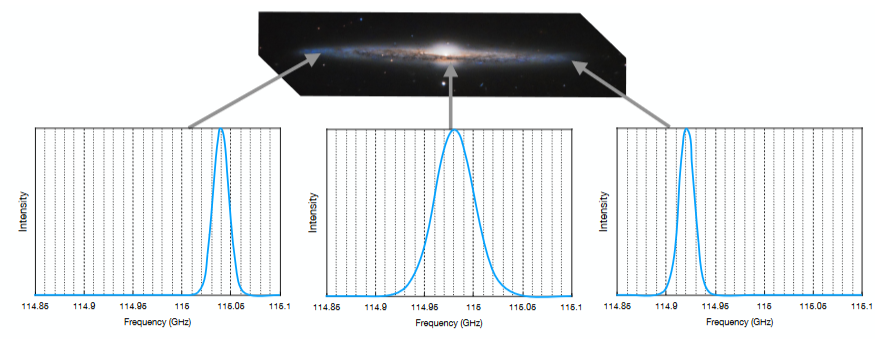
\includegraphics{C:/Users/maxst/sciencia/Pasted image 20211026113824.png}

We can determine the velocity, direction, and rotation of the galaxy
using the Doppler Shift formula:

\hypertarget{z-fracdeltalambdalambda_0}{%
\subsubsection{\texorpdfstring{{\[Z = \frac{\Delta\lambda}{\lambda_{0}}\]}}{Z = \textbackslash frac\{\textbackslash Delta\textbackslash lambda\}\{\textbackslash lambda\_\{0\}\}}}\label{z-fracdeltalambdalambda_0}}

...where {\(\Delta\lambda\)} is the \emph{change in wavelength} of the
shifted light, and {\(\lambda_{0}\)} is the '\emph{rest}' wavelength. By
converting the given frequencies into wavelengths, we can find the
observed Doppler shift of each of the three observations. The rest
wavelength can be obtained from the rest frequency, recalling that
{\(c = \nu\lambda\)}:

\hypertarget{lambda_0-fraccnu-frac299792458-ms115.27-times-109-hz-2.60078-times-10--3m.}{%
\subsubsection{\texorpdfstring{{\[\lambda_{0} = \frac{c}{\nu} = \frac{299,792,458\, m/s}{115.27 \times 10^{9}\, Hz} = 2.60078 \times 10^{- 3}m.\]}}{\textbackslash lambda\_\{0\} = \textbackslash frac\{c\}\{\textbackslash nu\} = \textbackslash frac\{299,792,458\textbackslash, m/s\}\{115.27 \textbackslash times 10\^{}\{9\}\textbackslash, Hz\} = 2.60078 \textbackslash times 10\^{}\{- 3\}m.}}\label{lambda_0-fraccnu-frac299792458-ms115.27-times-109-hz-2.60078-times-10--3m.}}

The spectra show transition frequencies of
{\(\nu_{1},\nu_{2},\nu_{3} = 115.04\, GHz,\, 114.97\, GHZ,\text{~and~}114.92\, GHz\)}
(left to right). We can find the corresponding wavelengths in identical
fashion:

\hypertarget{beginmatrix-lambda_1-fraccnu_1-2.60598-times-10--3-m.-lambda_2-fraccnu_2-2.60757-times-10--3-m.-lambda_3-fraccnu_3-2.60871-times-10--3-m.-endmatrix}{%
\subsubsection{\texorpdfstring{{\[\begin{matrix}
{\lambda_{1} = \frac{c}{\nu_{1}}} & {= 2.60598 \times 10^{- 3}\, m.} \\
{\lambda_{2} = \frac{c}{\nu_{2}}} & {= 2.60757 \times 10^{- 3}\, m.} \\
{\lambda_{3} = \frac{c}{\nu_{3}}} & {= 2.60871 \times 10^{- 3}\, m.} \\
\end{matrix}\]}}{\textbackslash begin\{matrix\}
\{\textbackslash lambda\_\{1\} = \textbackslash frac\{c\}\{\textbackslash nu\_\{1\}\}\} \& \{= 2.60598 \textbackslash times 10\^{}\{- 3\}\textbackslash, m.\} \textbackslash\textbackslash{}
\{\textbackslash lambda\_\{2\} = \textbackslash frac\{c\}\{\textbackslash nu\_\{2\}\}\} \& \{= 2.60757 \textbackslash times 10\^{}\{- 3\}\textbackslash, m.\} \textbackslash\textbackslash{}
\{\textbackslash lambda\_\{3\} = \textbackslash frac\{c\}\{\textbackslash nu\_\{3\}\}\} \& \{= 2.60871 \textbackslash times 10\^{}\{- 3\}\textbackslash, m.\} \textbackslash\textbackslash{}
\textbackslash end\{matrix\}}}\label{beginmatrix-lambda_1-fraccnu_1-2.60598-times-10--3-m.-lambda_2-fraccnu_2-2.60757-times-10--3-m.-lambda_3-fraccnu_3-2.60871-times-10--3-m.-endmatrix}}

We can see already that the wavelengths at all three locations all
exceed the rest wavelength - therefore, the light from the galaxy is
\textbf{redshifted} and we can conclude the galaxy is moving away from
us. We can relate the Doppler shift to the velocity of the galaxy with
the following (non-relativistic) relation:

\hypertarget{z-fracdeltalambdalambda_0-fracvclongrightarrow-v-cz.}{%
\subsubsection{\texorpdfstring{{\[Z = \frac{\Delta\lambda}{\lambda_{0}} = \frac{v}{c}\;\Longrightarrow\; v = cZ.\]}}{Z = \textbackslash frac\{\textbackslash Delta\textbackslash lambda\}\{\textbackslash lambda\_\{0\}\} = \textbackslash frac\{v\}\{c\}\textbackslash;\textbackslash Longrightarrow\textbackslash; v = cZ.}}\label{z-fracdeltalambdalambda_0-fracvclongrightarrow-v-cz.}}

Since the galaxy is rotating, each side will be moving away from us at a
different rate - one will move away faster than the center, and the
other will move away slower than the center. If we use the wavelength
from light at the \emph{center of the galaxy} ({\(\lambda_{2}\)}) in the
above relation, it should give us the velocity of the galaxy as a whole
with respect to us. The redshift at the center is:

\hypertarget{z-fracdeltalambdalambda_0-frac2.60757-times-10--3---2.60078-times-10--32.60078-times-10--3-0.00260938}{%
\subsubsection{\texorpdfstring{{\[Z = \frac{\Delta\lambda}{\lambda_{0}} = \frac{(2.60757 \times 10^{- 3} - 2.60078 \times 10^{- 3})}{2.60078 \times 10^{- 3}} = 0.00260938\]}}{Z = \textbackslash frac\{\textbackslash Delta\textbackslash lambda\}\{\textbackslash lambda\_\{0\}\} = \textbackslash frac\{(2.60757 \textbackslash times 10\^{}\{- 3\} - 2.60078 \textbackslash times 10\^{}\{- 3\})\}\{2.60078 \textbackslash times 10\^{}\{- 3\}\} = 0.00260938}}\label{z-fracdeltalambdalambda_0-frac2.60757-times-10--3---2.60078-times-10--32.60078-times-10--3-0.00260938}}

Plugging this into the velocity relation above, we find the velocity of
the galaxy to be:

\begin{quote}
\hypertarget{beginmatrix-v-cz-299792458textms-cdot-0.00260938-782271textms-782.271textkmsquadtextaway-from-us.quad-endmatrix}{%
\subsubsection{\texorpdfstring{{\[\begin{matrix}
v & {= cZ} \\
 & {= (299792458\text{m/s}) \cdot (0.00260938)} \\
 & {= 782,271\,\text{m/s}} \\
 & {= 782.271\,\text{km/s}\quad\text{away\ from\ us.}\quad} \\
\end{matrix}\]}}{\textbackslash begin\{matrix\}
v \& \{= cZ\} \textbackslash\textbackslash{}
 \& \{= (299792458\textbackslash text\{m/s\}) \textbackslash cdot (0.00260938)\} \textbackslash\textbackslash{}
 \& \{= 782,271\textbackslash,\textbackslash text\{m/s\}\} \textbackslash\textbackslash{}
 \& \{= 782.271\textbackslash,\textbackslash text\{km/s\}\textbackslash quad\textbackslash text\{away\textbackslash{} from\textbackslash{} us.\}\textbackslash quad\} \textbackslash\textbackslash{}
\textbackslash end\{matrix\}}}\label{beginmatrix-v-cz-299792458textms-cdot-0.00260938-782271textms-782.271textkmsquadtextaway-from-us.quad-endmatrix}}
\end{quote}

The non-relativistic equation holds in this case since the velocity
{\(v\operatorname{<<}c\)}. This is the \textbf{recession velocity} of
the galaxy, {\(v_{\text{recession}}\)}.

Take the \emph{rest frame of the galaxy} to be a coordinate system fixed
in the center of the galaxy such that the center of the galaxy is
stationary.

We can find the redshift in this rest frame by subtracting the redshift
of the center point ({\(Z_{2}\)}) from the redshifts of all three
points, eliminating the redshift caused by the relative motion of the
entire galaxy away from us. Doing this, we find the new values for
{\(Z\)} to be:

\hypertarget{beginmatrix-z_1-fracdeltalambda_1lambda_0---z_2---0.000610072.-z_2-0.-z_3-fracdeltalambda_3lambda_0---z_2-0.000436221.-endmatrix}{%
\subsubsection{\texorpdfstring{{\[\begin{matrix}
{Z_{1} = \frac{\Delta\lambda_{1}}{\lambda_{0}} - Z_{2}} & {= - 0.000610072.} \\
Z_{2} & {= 0.} \\
{Z_{3} = \frac{\Delta\lambda_{3}}{\lambda_{0}} - Z_{2}} & {= 0.000436221.} \\
\end{matrix}\]}}{\textbackslash begin\{matrix\}
\{Z\_\{1\} = \textbackslash frac\{\textbackslash Delta\textbackslash lambda\_\{1\}\}\{\textbackslash lambda\_\{0\}\} - Z\_\{2\}\} \& \{= - 0.000610072.\} \textbackslash\textbackslash{}
Z\_\{2\} \& \{= 0.\} \textbackslash\textbackslash{}
\{Z\_\{3\} = \textbackslash frac\{\textbackslash Delta\textbackslash lambda\_\{3\}\}\{\textbackslash lambda\_\{0\}\} - Z\_\{2\}\} \& \{= 0.000436221.\} \textbackslash\textbackslash{}
\textbackslash end\{matrix\}}}\label{beginmatrix-z_1-fracdeltalambda_1lambda_0---z_2---0.000610072.-z_2-0.-z_3-fracdeltalambda_3lambda_0---z_2-0.000436221.-endmatrix}}

In the rest frame, the center of the galaxy does not experience any
Doppler shift (since it is not moving relative to the frame). The left
point is \textbf{blueshifted} relative to the center - therefore, it is
rotating towards us, while the right point is still redshifted, moving
away from us. Therefore, the galaxy is rotating counter-clockwise
relative to a vertical axis perpendicular to the disk.

The following formula relates the \textbf{rotational velocity}
{\(v_{\text{rotation}}\)} to the \textbf{recession velocity}
{\(v_{\text{recession}}\)}:

\begin{quote}
\hypertarget{v_textrotation-fracv_los---v_textrecessionsini}{%
\subsubsection{\texorpdfstring{{\[v_{\text{rotation}} = \frac{v_{LOS} - v_{\text{recession}}}{\sin(i)}\]}}{v\_\{\textbackslash text\{rotation\}\} = \textbackslash frac\{v\_\{LOS\} - v\_\{\textbackslash text\{recession\}\}\}\{\textbackslash sin(i)\}}}\label{v_textrotation-fracv_los---v_textrecessionsini}}

where:

\begin{itemize}
\tightlist
\item
  {\(v_{LOS}\)} is the total radial velocity relative to the observer
  (found via Doppler Shift)
\item
  {\(i\)} is the \textbf{inclination} angle of the galaxy relative to
  the observer.
\end{itemize}
\end{quote}

From the figure, we assume that the inclination angle {\(i\)} is
90{\({^\circ}\)} (viewed edge-on, like the side of a plate), so the
denominator reduces to 1. We can now pick one of our points on the edge
of the galaxy to find the rotational velocity. Taking the rightmost
point:

\hypertarget{v_los-cz_3-913047textms.}{%
\subsubsection{\texorpdfstring{{\[v_{LOS} = cZ_{3} = 913047\text{~m/s.}\]}}{v\_\{LOS\} = cZ\_\{3\} = 913047\textbackslash text\{\textasciitilde m/s.\}}}\label{v_los-cz_3-913047textms.}}

Therefore:

\begin{quote}
\hypertarget{v_textrotation-v_los---v_textrecession-130776textms.}{%
\subsection{\texorpdfstring{{\[v_{\text{rotation}} = v_{LOS} - v_{\text{recession}} = 130,776\text{~m/s}.\]}}{v\_\{\textbackslash text\{rotation\}\} = v\_\{LOS\} - v\_\{\textbackslash text\{recession\}\} = 130,776\textbackslash text\{\textasciitilde m/s\}.}}\label{v_textrotation-v_los---v_textrecession-130776textms.}}
\end{quote}

\textbf{NB}: the rotational velocity of the galaxy is not constant - the
gas on the other side of the galaxy (left), for which we measured a
slightly different Doppler shift ({\(Z_{1}\)}), will have a different
{\(v_{\text{rotation}}\)}. To find the total angular velocity of the
galaxy as a whole, more information is required (eg. distances, mass).

\begin{center}\rule{0.5\linewidth}{0.5pt}\end{center}

\hypertarget{section}{%
\subsubsection{3.}\label{section}}

This question illustrates how we can use parallax and observations of
the general/average properties of stars to "bootstrap" other methods,
thereby determining distances to objects that are even further away.
Ignore all interstellar extinction in this question.

\begin{center}\rule{0.5\linewidth}{0.5pt}\end{center}

\textbf{a.} You observe a star and determine its parallax to be
{\(5.37\)} milliarcseconds. From photometery (measuring light
intensity), you determine its apparent visual magnitude to be
{\(m_{v} = + 0.50\)}, and its apparent blue magnitude to be
{\(m_{B} = + 2.35\)}. From spectroscopy you determine that this is a
\emph{red supergiant} star. Calculate the absolute visual and blue
magnitudes ({\(M_{v}\)} and {\(M_{b}\)}) of this star.

First, we use the measured parallactic angle to find the distance to the
star. Assuming the parallax was measured with a baseline of {\(1\, AU\)}
(maximum separation in Earth's orbit), we can find the distance via the
following relation:

\hypertarget{beginmatrix-dtextpc-frac1ptext-frac15.37-times-10--3-186.22textpc.-endmatrix}{%
\subsubsection{\texorpdfstring{{\[\begin{matrix}
{D\text{~(pc)}} & {= \frac{1}{p\text{~(")}}} \\
 & {= \frac{1}{5.37 \times 10^{- 3}}} \\
 & {= 186.22\text{~pc}.} \\
\end{matrix}\]}}{\textbackslash begin\{matrix\}
\{D\textbackslash text\{\textasciitilde(pc)\}\} \& \{= \textbackslash frac\{1\}\{p\textbackslash text\{\textasciitilde(")\}\}\} \textbackslash\textbackslash{}
 \& \{= \textbackslash frac\{1\}\{5.37 \textbackslash times 10\^{}\{- 3\}\}\} \textbackslash\textbackslash{}
 \& \{= 186.22\textbackslash text\{\textasciitilde pc\}.\} \textbackslash\textbackslash{}
\textbackslash end\{matrix\}}}\label{beginmatrix-dtextpc-frac1ptext-frac15.37-times-10--3-186.22textpc.-endmatrix}}

Now that we have the distance in parsecs, we can use the \emph{distance
modulus} to relate the apparent magnitudes to the absolute magnitudes
using the following relation:

\hypertarget{m---m-5loglbrack-drbrack---5}{%
\subsubsection{\texorpdfstring{{\[m - M = 5\log\lbrack D\rbrack - 5\]}}{m - M = 5\textbackslash log\textbackslash lbrack D\textbackslash rbrack - 5}}\label{m---m-5loglbrack-drbrack---5}}

...where the little {\(m\)} is the apparent magnitude, and the large
{\(M\)} is the absolute magnitude. Subsituting the given values of
{\(m_{b}\)} and {\(m_{v}\)} into the formula, we find the absolute
magnitudes to be:

\begin{quote}
\hypertarget{beginmatrix-m_v-m_v---5loglbrack-drbrack-5-0.50---5loglbrack-186.22rbrack-5---5.85013-m_b-m_b---5loglbrack-drbrack-5-2.35---5loglbrack-186.22rbrack-5---4.00013-endmatrix}{%
\subsubsection{\texorpdfstring{{\[\begin{matrix}
M_{v} & {= m_{v} - 5\log\lbrack D\rbrack + 5} \\
 & {= 0.50 - 5\log\lbrack 186.22\rbrack + 5} \\
 & {= - 5.85013} \\
M_{b} & {= m_{b} - 5\log\lbrack D\rbrack + 5} \\
 & {= 2.35 - 5\log\lbrack 186.22\rbrack + 5} \\
 & {= - 4.00013} \\
\end{matrix}\]}}{\textbackslash begin\{matrix\}
M\_\{v\} \& \{= m\_\{v\} - 5\textbackslash log\textbackslash lbrack D\textbackslash rbrack + 5\} \textbackslash\textbackslash{}
 \& \{= 0.50 - 5\textbackslash log\textbackslash lbrack 186.22\textbackslash rbrack + 5\} \textbackslash\textbackslash{}
 \& \{= - 5.85013\} \textbackslash\textbackslash{}
M\_\{b\} \& \{= m\_\{b\} - 5\textbackslash log\textbackslash lbrack D\textbackslash rbrack + 5\} \textbackslash\textbackslash{}
 \& \{= 2.35 - 5\textbackslash log\textbackslash lbrack 186.22\textbackslash rbrack + 5\} \textbackslash\textbackslash{}
 \& \{= - 4.00013\} \textbackslash\textbackslash{}
\textbackslash end\{matrix\}}}\label{beginmatrix-m_v-m_v---5loglbrack-drbrack-5-0.50---5loglbrack-186.22rbrack-5---5.85013-m_b-m_b---5loglbrack-drbrack-5-2.35---5loglbrack-186.22rbrack-5---4.00013-endmatrix}}
\end{quote}

\begin{center}\rule{0.5\linewidth}{0.5pt}\end{center}

\textbf{b.} Assuming that \emph{every} red supergiant star in the
universe has similar properties, and therefore the same {\(M_{v}\)} and
{\(M_{b}\)} (which happens to be a relatively good assumption), you now
find another red supergiant in the Large Magellanic Cloud, a dwarf
galaxy orbiting our own. For this star, you measure {\(m_{v}\)} and
{\(m_{b}\)} to be {\(12.55\)} and {\(14.40\)}, respectively. Calculate
the distance to the LMC (\emph{in pc}).

We have {\(M_{v},\, M_{b} = - 5.85013, - 4.00013\)} respectively. We can
rearrange the previous equation:

\begin{quote}
\hypertarget{m---m-5loglbrack-drbrack-5}{%
\subsubsection{\texorpdfstring{{\[m - M = 5\log\lbrack D\rbrack + 5\]}}{m - M = 5\textbackslash log\textbackslash lbrack D\textbackslash rbrack + 5}}\label{m---m-5loglbrack-drbrack-5}}

\hypertarget{fracm---m---55-loglbrack-drbrack}{%
\subsubsection{\texorpdfstring{{\[\frac{m - M - 5}{5} = \log\lbrack D\rbrack\]}}{\textbackslash frac\{m - M - 5\}\{5\} = \textbackslash log\textbackslash lbrack D\textbackslash rbrack}}\label{fracm---m---55-loglbrack-drbrack}}

\hypertarget{d-1015m---m---5}{%
\subsubsection{\texorpdfstring{{\[D = 10^{(1/5)(m - M - 5)}\]}}{D = 10\^{}\{(1/5)(m - M - 5)\}}}\label{d-1015m---m---5}}
\end{quote}

Substituting our values for {\(m_{b},M_{b}\)} into this equation, we
find the distance to be:

\begin{quote}
\hypertarget{d_b-1015m_b---m_b---5-101514.40-4.00013---5-478.659-pc.}{%
\subsubsection{\texorpdfstring{{\[D_{b} = 10^{(1/5)(m_{b} - M_{b} - 5)} = 10^{(1/5)(14.40 + 4.00013 - 5)} = 478.659\, pc.\]}}{D\_\{b\} = 10\^{}\{(1/5)(m\_\{b\} - M\_\{b\} - 5)\} = 10\^{}\{(1/5)(14.40 + 4.00013 - 5)\} = 478.659\textbackslash, pc.}}\label{d_b-1015m_b---m_b---5-101514.40-4.00013---5-478.659-pc.}}
\end{quote}

Doing the same for {\(m_{v},M_{v}\)}:

\begin{quote}
\hypertarget{d_v-1015m_v---m_v---5-101512.55-5.85013---5-478.659-pc.}{%
\subsubsection{\texorpdfstring{{\[D_{v} = 10^{(1/5)(m_{v} - M_{v} - 5)} = 10^{(1/5)(12.55 + 5.85013 - 5)} = 478.659\, pc.\]}}{D\_\{v\} = 10\^{}\{(1/5)(m\_\{v\} - M\_\{v\} - 5)\} = 10\^{}\{(1/5)(12.55 + 5.85013 - 5)\} = 478.659\textbackslash, pc.}}\label{d_v-1015m_v---m_v---5-101512.55-5.85013---5-478.659-pc.}}
\end{quote}

The results agree (as expected), so we can conclude that the distance to
the LMC is {\(478.659\, pc.\)}

\begin{center}\rule{0.5\linewidth}{0.5pt}\end{center}

\textbf{c.} The physical mechanism that produces a supernova results in
every supernova having approximately the same \emph{luminosity}. Assume
you now see a supernova explosion in the LMC and measure
{\(m_{v} = - 0.77\)}. Calculate the absolute visual magnitude of this
supernova (and therefore, the value of {\(M_{v}\)} for every supernova
in the universe).

Using the same relation as the previous question:

\hypertarget{beginmatrix-m_v-m_v---5loglbrack-drbrack-5---0.77---5loglbrack-478.659rbrack-5---9.17013-endmatrix}{%
\subsubsection{\texorpdfstring{{\[\begin{matrix}
M_{v} & {= m_{v} - 5\log\lbrack D\rbrack + 5} \\
 & {= - 0.77 - 5\log\lbrack 478.659\rbrack + 5} \\
 & {= - 9.17013} \\
\end{matrix}\]}}{\textbackslash begin\{matrix\}
M\_\{v\} \& \{= m\_\{v\} - 5\textbackslash log\textbackslash lbrack D\textbackslash rbrack + 5\} \textbackslash\textbackslash{}
 \& \{= - 0.77 - 5\textbackslash log\textbackslash lbrack 478.659\textbackslash rbrack + 5\} \textbackslash\textbackslash{}
 \& \{= - 9.17013\} \textbackslash\textbackslash{}
\textbackslash end\{matrix\}}}\label{beginmatrix-m_v-m_v---5loglbrack-drbrack-5---0.77---5loglbrack-478.659rbrack-5---9.17013-endmatrix}}

\begin{center}\rule{0.5\linewidth}{0.5pt}\end{center}

\textbf{d.} Now you observe a supernova explosion (with
{\(m_{v} = 14.33\)}) in a distant galaxy. Calculate the distance to this
galaxy (\emph{in {\(Mpc\)}}).

\begin{center}\rule{0.5\linewidth}{0.5pt}\end{center}

\textbf{e.} The Hubble Law is a simple formula relating the redshifted
velocity of a galaxy to its distances:
{\(V\text{~(km/s)} = H_{0}\, D\,(Mpc).\)}, originating from the fact
that the universe is expanding. {\(H_{0}\)} is the \textbf{Hubble
Constant}, and has units of {\(km/s \cdot Mpc^{- 1}\)}. In the galaxy
from part \textbf{d.}, you observe a hydrogen spectrum at a wavelength
of {\(664.9916\text{~nm}\)}. The rest wavelength of hydrogen is
{\(656.000\text{~nm}.\)} Calculate the value of the Hubble Constant.

\begin{center}\rule{0.5\linewidth}{0.5pt}\end{center}

\textbf{f.} Finally, you observe a galaxy that is too far away to see
any individual stars and does not have a supernova in it. But you take a
spectrum of this galaxy and find that the hydrogen spectrum (which
should be at {\(656.00\text{~nm}\)}) is actually at a wavelength of
{\(2.00\,\mu m\)}. Using your results from \textbf{e}, calculate the
distance to this galaxy (\emph{in {\(Mpc\)}}).

\begin{center}\rule{0.5\linewidth}{0.5pt}\end{center}

\end{document}
